\documentclass[12pt,letterpaper]{report}

%\usepackage{wordlike}

\usepackage{amsmath}
\usepackage{amsfonts}
\usepackage{amssymb}
\usepackage{graphicx}
\usepackage{tabularx}
%\usepackage{algorithmic}
\usepackage{algorithm,algpseudocode}
\usepackage{csquotes}
\usepackage{subcaption}
\usepackage[font=small]{caption}
\usepackage{url}
\usepackage[english]{babel}
\usepackage{setspace} 
\usepackage[margin=1in]{geometry}

\usepackage[hidelinks]{hyperref}

\usepackage{sectsty}
\allsectionsfont{\normalsize\textbf\bfseries}



%\usepackage{titlesec}
%\titleformat{\chapter}[frame]{\normalfont\fontsize{12}{15}}{\thechapter}




%\usepackage{times}
%\usepackage{venturis2}

\doublespacing

\title{\textsc{BUILDING ROBUST DISTRIBUTED INFRASTRUCTURE NETWORKS}}
\author{\textsc{Brendan Lane Benshoof}}
\date{}

\begin{document}
	
	\pagenumbering{gobble}

	
	\begin{center}
		%	\includegraphics[width=0.15\textwidth]{example-image-1x1}\par\vspace{1cm}
		{\scshape BUILDING ROBUST DISTRIBUTED INFRASTRUCTURE NETWORKS\par}
		\vspace{0.5cm}
		{by\par}
		\vspace{0.5cm}
		{\scshape Brendan Lane Benshoof\par}
		\vspace{0.5cm}
		{Under the Direction of ~Robert ~Harrison \par}
		\vspace{0.5cm}
		{\scshape Abstract \par}
		
	\end{center}
	
	Many competing designs for Distributed Hash Tables exist exploring multiple models of addressing, routing and network maintenance. 
Designing a general theoretical model and implementation of a Distributed Hash Table allows exploration of the possible properties of distributed hash tables. We will propose a generalized model of DHT behavior, centered on utilizing Delunay triangulation in a given metric space to maintain the network’s topology. We will show that utilizing this model, we can produce network typologies that approximate existing DHT methods and provide a starting point for further exploration.
Previous research has explored utilizing a hyperbolic metric space to provide efficient greedy routing for overlay networks. We will use our generalized model of DHT construction to design and implement more efficient distributed hash table protocol, and discuss the qualities of potential successors to existing DHT technologies.
	
	\vfill
	
	
	% Bottom of the page

	
	
	\newpage 
	\begin{titlepage}
		
		\begin{center}
			%	\includegraphics[width=0.15\textwidth]{example-image-1x1}\par\vspace{1cm}
			{\scshape BUILDING ROBUST DISTRIBUTED INFRASTRUCTURE NETWORKS\par}
			\vspace{5cm}
			{by\par}
			\vspace{5cm}
			{\scshape Brendan Lane Benshoof\par}
			
			\vfill
			A Dissertation Submitted in Partial Fulfillment of the Requirements for the Degree of\\
			Doctor of Philosophy\\
			in the College of Arts and Sciences\\
			Georgia State University\\
			2016
		\end{center}
	\end{titlepage}
	
	
	
	
	
	
	\null\vfill
	\begin{center}
		
		Copyright by \\
		Brendan Lane Benshoof\\
		2016
	\end{center}
	\newpage
	
	
	
	\begin{center}
		{\scshape BUILDING ROBUST DISTRIBUTED INFRASTRUCTURE NETWORKS\par}
		\vspace{5cm}
		{by\par}
		\vspace{5cm}
		{\scshape Brendan Lane Benshoof\par}
	\end{center}
	\vfill
	\hfill\begin{tabular}{rl}
		Committee Chair & Robert Harrison \\ 
		&  \\ 
		Committee &  Raj Sunderraman \\ 
		& Anu G. Bourgeois\\ 
		& Valerie Miller 
	\end{tabular} 
	
	
	\noindent
	Electronic Version Approved:\\
	\vspace{1cm}
	
	\noindent
	Office of Graduate Studies \\
	College of Arts and Sciences \\
	Georgia State University\\
	May 2016 
	
	
	
	
	\chapter*{Dedication}
	This work is dedicated to those in my who supported me in pursuing my education out of a desire to see me grow: my patient and encouraging spouse, Erin Gillman, and my parents, Bill and Denise Benshoof, who have been active sponsors of my education for my entire life.
	
	
	\chapter*{Acknowledgements}	

\begin{itemize}
\item	Dr. Michael Weeks, who introduced me to the possibility of graduate school, teaching, and research.
\item	Dr. Valerie Miller, who encouraged my curiosity and has always pushed me to do more. 
\item	Dr. Raj Sunderraman, who encouraged me to attend Georgia State and helped my find my role here.
\item	Dr. Anu Bourgeois, who fostered my interest in networking and distributed systems.
\item	Dr. Robert Harrison, who has been my teacher, sponsor and mentor.
\item   Andrew Rosen, who has been my serial co-author and good friend.
\end{itemize}
	

	
	\setcounter{tocdepth}{0}
	\tableofcontents
	\cleardoublepage
	\pagenumbering{roman}


	\setcounter{tocdepth}{1}
	\listoftables
	\addcontentsline{toc}{chapter}{List of Tables}
	\listoffigures
	\addcontentsline{toc}{chapter}{List of Figures}
	
	%\addcontentsline{toc}{chapter}{\listtablename}
	%\addcontentsline{toc}{chapter}{\listfigurename}
	

	\clearpage	
	
	
	\pagenumbering{arabic}
	





\chapter{Introduction}

As more and more systems are growing using existing P2P technology, we are building services usable by the public (and exploring even more possibilities) based on a P2P system called a Distributed Hash Table.
While current Distributed Hash Tables are incredible effective and robust solution to maintain a shared state in a P2P system in a scalable fashion, little to no improvement has been provided over the initial Chord\cite{chord} and Kademlia\cite{kademlia} DHTs.
This dissertation explores improvements and applications of Distributed Hash Tables to provide the capacity for future robust and distributed systems infrastructures and services.

\section{The Ship of Theseus}

\singlespacing
\blockquote{The ship wherein Theseus and the youth of Athens returned from Crete had thirty oars, and was preserved by the Athenians down even to the time of Demetrius Phalereus, for they took away the old planks as they decayed, putting in new and stronger timber in their places, in so much that this ship became a standing example among the philosophers, for the logical question of things that grow; one side holding that the ship remained the same, and the other contending that it was not the same.

-Plutarch, Theseus

}
\doublespacing

What has attracted me to the design and applications of Distributed Hash Tables is that they encourage thinking on a global scale and require designs that operate with minimal human intervention on time scales beyond those normally considered by computer science.
In traditional engineering and design we conceive of an object, that while having parts replaced in the course of maintenance, will largely remain a single static object comprised of the same material of which it was formed until it is disposed of.
When considering a Distributed Hash Table, we are intentionally designing a system like the Ship of Theseus, where on the scale of millions of devices are added and lost on a daily basis, often amounting to up to half of the constituent parts of a globe spanning system being replaced in a day.
It is our task to design a pattern of behavior for each of these parts that allows the system to respond to queries despite constant in-progress failure and replacement and to constantly propagate the information stored in the system onward to new storage before the current storage fails. 

Despite the challenge involved in building such a system, barring dramatic change to our expectations of the future, the existing Distributed Hash Tables will be able to persist as a public utility indefinitely.
I present that the answer to the Paradox of the Ship of Theseus is, "I don't care as long as the ship still floats".

\section{Goals}

The goals of the papers making up this dissertation are straightforward.
Four subjects concerning DHTs are open and meriting improvement, generalization, application, efficiency, and robustness. 
\begin{itemize}

\item DGVH and UrDHT present ideas to generalize our model of "What is a Distributed Hash Table" beyond the current proposed methods into a continuum of viable DHT methods which we can explore for ideal properties. 

\item ChordReduce is concerned with application of a DHT to act as an organizing mechanism for a traditional distributed computing paradigm, but with viability at larger scales of operation and duration.

\item Hyperbolic DHTs utilize the generalized model of distributed hash tables to realize the idea of using a hyperbolic coordinate space to improve DHT efficiency that has existed in theory for about a decade.

\item New replication strategies will allow DHTs to store records with essentially zero loss on any time scale the implementers deem appropriate for their uses. 


\end{itemize}



\chapter{Technical Background}
\section{What is a DHT?}
At the core of maintaining a distributed system is establishing a shared state in the form of a table of key-value pairs.
DHTs provide a mechanism for agreeing upon a very large shared state with tolerable inconsistency (records are sometimes lost, and if mutable they may be inconsistent in value).
While other techniques of consensus provide higher confidence, DHTs scale to awesome levels of storage capacity because they are highly tolerant of the failure of nodes within themselves.
In practice, DHTs and similar distributed systems' performance are bound by the CAP Theorem\cite{brewer2010certain}.

\subsection{CAP Theorem/ Brewer’s Theorem}
CAP Theorem describes a trade-off between three Attributes of distributed systems.
It states that any distributed system is a compromise between consistency, availability and partition tolerance and that no distributed store of state can posses all of these qualities at a time.
\begin{itemize}
\item Consistency: Everybody agrees on the contents of shared data
\item Availability: Everybody can quickly and consistently access all the data.
\item Partition Tolerance: The network can handle loss of nodes and connectivity between nodes without loosing the system's cohesion or data.
\end{itemize}

As partition tolerance is required in a DHT for long term operation, this leaves us a trade-off between Consistency and Availability.
In DHTs consistency is limited to assure availability of records to users, however such trade-offs are not binary, and we can can seek a balance between availability and consistency to best suit the needs of applications.


\section{What are the currently existing DHTs?}

Chord and Kademlia are the most commonly used DHTs in practice. 
Chord has been favored by researchers because it was designed with a series of proofs to show its consistency in the face of churn.
Sadly these proofs have been shown to be incorrect\cite{zave2012using} without serious modification to the established protocol.


\subsection{Chord}
Chord\cite{chord} is a peer-to-peer (P2P) protocol for file sharing and distributed storage that guarantees a high probability $\log_{2} N$  lookup time for a particular node or file in a network with N nodes. 
It is highly fault-tolerant to node failures and churn, the constant joining and leaving of nodes.  It scales extremely well and the network requires little maintenance to handle individual nodes.  
Files in the network are distributed evenly among its members.

As a distributed hash table (DHT), each member of the network and the data stored on the network is mapped to a unique $m$-bit key or ID, corresponding to one of  $2^m$ locations on a ring. 
The ID of a node and the node itself are referred to interchangeably.

In a traditional Chord network, all messages travel in one direction - upstream, hopping from one node to another with a greater ID until it wraps around.
A node in the network is responsible for all the data with keys \textit{above or upstream} his predecessor, up through and including its own ID.  If a node is responsible for some key, it is referred to as being the successor of that key.

Robustness in the network is accomplished by having nodes backup their contents to their $s$ (often 1) immediate successors, the closest nodes upstream.  
This is done because when a node leaves the network or fails, the most immediate successor would be responsible for the content its content.

Each node maintains a table of $m$ shortcuts to other peers, called the finger table.   The $i$th entry of a node $n$'s finger table corresponds to the node that is the successor of the key $n+2^{i-1} \mod 2^m $.  
Nodes route messages to the finger that is closest to the sought key without going past it, until it is received by the responsible node.  This provides Chord with a highly scalable $\log_2(N)$ lookup time for any key\cite{chord}.

As nodes enter and leave the ring, the nodes use their maintenance procedures to guide them into the right place and repair any links with failed nodes.  Full details on Chord's maintenance cycle are beyond the scope of this paper and can be found here\cite{chord}.

\begin{figure}
	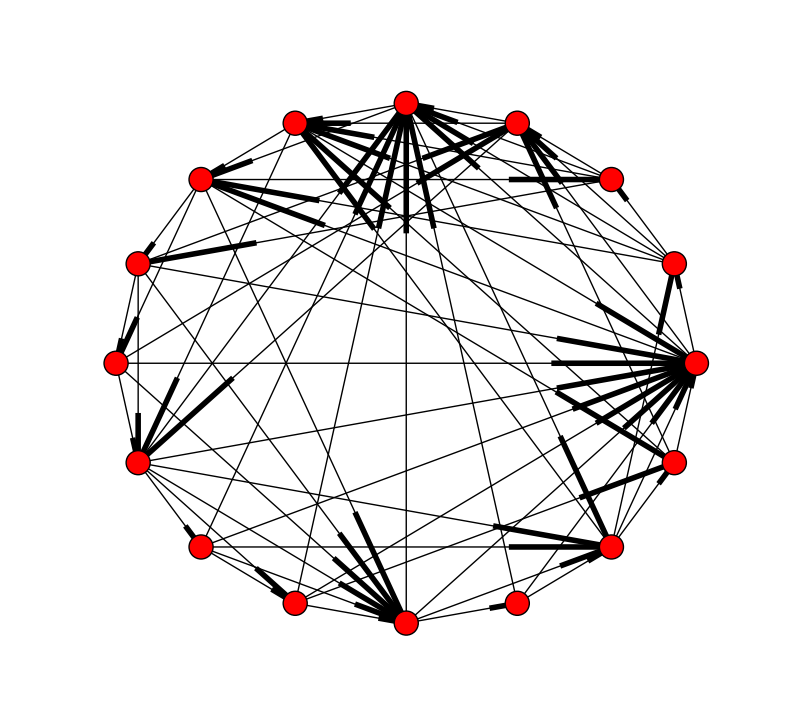
\includegraphics[width=0.5\linewidth]{chordreal}
	\caption{A Chord ring 16 nodes where $m=4$.  The bold lines are incoming edges.  Each node has a connection to its successor, as well as 4 fingers, some of which are duplicates.}
	\label{chordreal}
\end{figure}


\subsection{Kademlia}

Kademlia is the most popular DHT methodology. 
It powers the trackerless bittorent mainline DHT, and the C implementation related to that project is likely the greatest cause of its popularity.
Many other distributed systems utilize modified versions of Kademlia as a means of peer management and as a key-value store.

Kademlia is built in a non-Eucldian metric space. 
Locations are represented by a large integer (160 bit is most common) and the distance between locations is calculated by the XOR metric.
This means Kademlia's metric space is a generalization of a binary tree, where the locations are mapped to leaf nodes and distance between nodes is the distance required to traverse between them on that tree.

Because of the geometric awkwardness of its metric, Kademlia uses a modified k-nearest neighbors approach to approximate node's Voronoi regions and Delaunay peers.
If nodes are evenly distributed through the space, Kademlia's metric provides an $O(log(n))$ diameter network.


\section{What are DHTs used for}

DHTs are designed to be used to store data in a distributed system that would normally be centrally stored in other systems, like a database or other records.
In practice, they also double as a mechanism for peers discovery and network management.
Many P2P services use a DHT as part of their infrastructure: Bitorrent\cite{jimenez2011kademlia}, CJDNS\cite{hodson2013meshnet}, and I2P\cite{zantout2011i2p}
% %Give examples of how DHTs are used in those projects

	
\chapter{MapReduce on a Chord Distributed Hash Table}

\begin{center}
Andrew Rosen \qquad Brendan Benshoof  \qquad Robert W. Harrison \qquad Anu G. Bourgeois

Published ICA Conference 2014
\end{center}


\section{Introduction}

%\textit{The story we want to tell is that map reduce is awesome.  Here is alist of pros for ma reduce. Awesome but designed for data center use, which is a subset of the possible configuration but really the only one explored in depth. Introduce single point of failure and if we want to explore using mapreduce in  a more generalized manner we have to solve the problem of a single point of failure.  P2P frameworks are explicitly designed to eliminate single points of failure, scale, wax platonic on virtues of P2P. We were motivated to look at it from a more abstract point of view and ask how can we do map reduce jobs over a more generalized/distributed configuration.  THis paper presents ChordReduce}



Google's MapReduce \cite{mapreduce} paradigm has rapidly become an integral part in the world of data processing and is capable of efficiently executing numerous Big Data programming and data-reduction tasks.  By using MapReduce, a user can take a large problem, split it into small, equivalent tasks and send those tasks to other processors for computation.  The results are sent back to the user and combined into one answer.  MapReduce has proven to be an extremely powerful and versatile tool, providing the framework for using distributed computing to solve a wide variety of problems, such as distributed sorting and creating an inverted index \cite{mapreduce}. 


%Many popular platforms for MapReduce, such as Hadoop \cite{Hadoop}, utilize a central source of coordination and organization to store and operate on data. The hierarchical structure of Hadoop results in a single point of failure at the node that concentrates the results and also requires a complicated scheme for handling node failures.

Popular platforms for MapReduce, such as Hadoop \cite{Hadoop}, are explicitly designed to be used in large datacenters \cite{hadoopAssumptions} and the majority of research has been focused there.  
These MapReduce platforms are highly centralized and tend to have single points of failure\cite{shvachko2010hadoop} as a result.   A centralized design assumes that the network is relatively unchanging and does not usually have mechanisms to handle node failure during execution or, conversely, cannot speed up the execution of a job by adding additional workers on the fly.  Finally deploying these systems and developing programs for them has an extremely steep learning curve.


% http://wiki.apache.org/hadoop/Virtual%20Hadoop  <---- look here for motivation.
We were motivated to start exploring a more abstract deployment for MapReduce, one that could be deployed in a much wider variety of contexts, from peer-2-peer frameworks to datacenters.  Our framework cannot and does not rely on many common assumptions, such as a dedicated and static network of homogeneous machines. Nor do we assume that failed nodes will recover \cite{hadoopAssumptions}.  Finally, our framework needed to be easy to deploy and simple to use.    

We used Chord\cite{chord}, a peer-2-peer distributed hash table, as the backbone for developing our system.  Our paper presents these contributions:
\begin{itemize}
	\item We define the architecture and components of ChordReduce and demonstrate how they fit together to perform MapReduce jobs over a distributed system without the need of a central scheduler or coordinator, avoiding a central point of failure. We also demonstrate how to create programs to solve MapReduce problems using ChordReduce (Section III). 
	\item We built a prototype system implementing ChordReduce and deployed it on Amazon's Elastic Cloud Compute.  We tested our deployment by solving Monte-Carlo computations and word frequency counts on our network (Section IV).
	\item We prove that ChordReduce is scalable and highly fault tolerant, even under high levels of churn and can even benefit from churn under certain circumstances. Specifically, we show it is robust enough to reassign work during runtime in response to nodes entering and leaving the network (Section V).
	\item We contrast ChordReduce with similar architectures and identify future areas of fruitful research using ChordReduce (Sections  VI and VII). 





\end{itemize}
%While Chord could be used to implement a grid computing environment similar to BOINC \cite{boinc} or Folding@home \cite{folding}, it would be difficult to efficiently implement the MapReduce algorithm using grid computing tools. MapReduce uses persistent data to amortize the cost of distributing the data across the nodes over many calls, while grid environments typically transmit a transient bundle of data and computation to a volunteer node. BOINC and Folding@home use a master-slave architecture with a critical point of failure similar to Hadoop, while ChordReduce is a true peer-based approach.

\section{Background}
ChordReduce takes its name from the two components it is built upon.  Chord\cite{chord} provides the backbone for the network and the file system, providing scalable routing, distributed storage, and fault-tolerance.   MapReduce runs on top of the Chord network and utilizes the underlying features of the distributed hash table.  This section provides background on Chord and MapReduce.



\subsection{MapReduce}
At its core, MapReduce \cite{mapreduce} is a system for division of labor, providing a layer of separation between the programmer and the more complicated parts of concurrent processing.  The programmer sends a large task to a master node, who then divides that task among slave nodes (which may further divide the task).  This task has two distinct parts: Map and Reduce.  Map performs some operation on a set of data and then produces a result for each Map operation.  The resulting data can then be reduced, combining these sets of results into a single set, which is further combined with other sets.  This process continues until one set of data remains.  A key concept here is the tasks are distributed to the nodes that already contain the relevant data, rather than the data and task being distributed together among arbitrary nodes.

The archetypal example of using MapReduce is counting the occurrence of each word in a collection of documents, called WordCount.  These documents have been split up into blocks and stored on the network over the distributed file system.  The master node locates the worker nodes with blocks and sends the Map and Reduce tasks associated with WordCount.  Each worker then goes through their blocks and creates a small word frequency list.  These lists are then used by other workers, who combine them into larger and larger lists, until the master node is left with a word frequency list of all the words in the documents. 
%The master node splits up the documents into multiple blocks and sends them off to workers.  


The most popular platform for MapReduce is Hadoop \cite{Hadoop}. Hadoop is an open-source Java implementation developed by Apache and Yahoo! \cite{pavlo2009comparison}.  Hadoop has two components, the Hadoop Distributed File System (HDFS) \cite{hdfs} and the Hadoop MapReduce Framework \cite{mrsurvey}.  Under HDFS, nodes are arranged in a hierarchical tree, with a master node, called the NameNode, at the top.  The NameNode's job is to organize and distribute information to the slave nodes, called DataNodes.  This makes the NameNode a single point of failure \cite{shvachko2010hadoop} in the network, as well as a potential bottleneck for the system \cite{hadoop-bottle}.

To do work on Hadoop, the user stores their data on the network.  This is handled by the NameNode, which equally apportions the data among the DataNodes.  When a user wants to run some analysis on the data or some subset the data, then that function is sent by the NameNode to each of the DataNodes that is responsible for the indicated data.   After the DataNode finishes processing, the result is handled by other nodes called Reducers which collect and reduce the results of multiple DataNodes.


\section{ChordReduce}
\textit{While the subsections in this section are complete, this intro is a mess of cut and pasted text}
Popular platforms for MapReduce, such as Hadoop, are extremely powerful, but have some inherent limitations.  
These platforms are designed to be deployed in a data center.  
Their architecture relies on multiple nodes with specific roles to coordinate the work, such as the NameNode and JobTracker.
These nodes perform necessary scheduling and distribution tasks and help provide fault-tolerance to the network as a whole, but in doing so become single points of failure themselves.

ChordReduce is designed as a more abstract framework for MapReduce, able to run on any arbitrary distributed configuration.
ChordReduce leverages the features of distributed hash tables to handle distributed file storage, fault tolerance, and lookup.  We designed ChordReduce to ensure that no single node is a point of failure and that there is no need for any node to coordinate the efforts of other nodes during processing.  

%ChordReduce uses Chord to act as a completely distributed topology for MapReduce, negating the need to assign any explicit roles to nodes or have a scheduler or coordinator.  ChordReduce does not need to assign specific nodes the task of backing up work; nodes backup their tasks using the same process that would be used for any other data being sent around the ring.  Finally, results work their way back to a specified hash address, rather than a specific hash node, eliminating any single point of failure in the network.  These features help prevent a bottleneck from occurring. The result is a simple, distributed, and highly robust architecture for MapReduce.


Our central design philosophy was to implement additions to the Chord protocol by leveraging the existing features of Chord.  By treating each task or target computation as an object of data, we can distribute them in the same manner as files and rely on the protocol to route them and provide robustness.
%ChordReduce is a fully functional Chord implementation in Python, with the same topology and functionality.  Nodes join the ring by contacting an existing node and are integrated into the network  via each node's maintenance cycle.

\textit{\cite{leemap} says that latency is similar.}  Marozzo et al. \cite{marozzo2012p2p} shows that adding additional fault-tolerance features to a MapReduce architecture is worth the added cost of maintenance, as the time lost due to node failures is greatly reduced.

\begin{figure}
    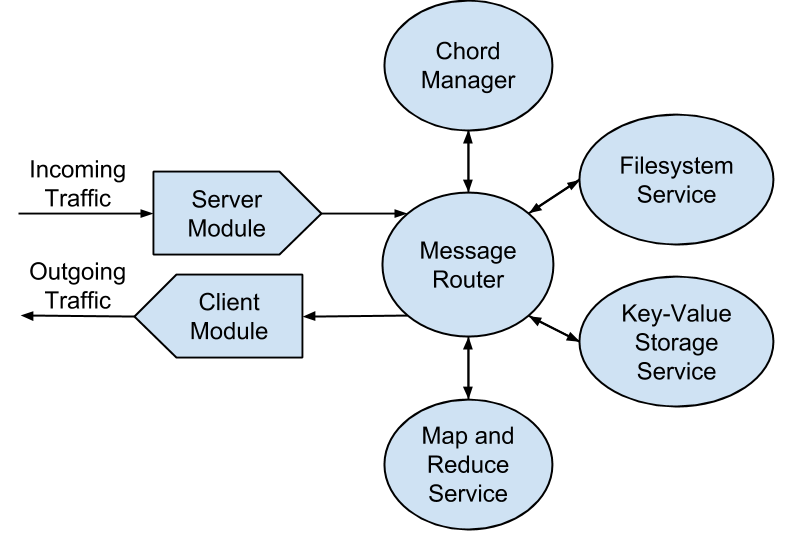
\includegraphics[width=\linewidth]{crArch}
    \caption{The basic architecture of a node in ChordReduce.  MapReduce runs as a service on top of each node.}
    \label{crArch}
\end{figure}




\textit{insert architecture layer diagram }  and \textit{insert work flow diagram.  Chord tree of stage, map , reduce.}
%ChordReduce is a fully functional Chord implementation in Python.  Our installation was designed to be as simple as possible.  It consists of downloading our code \cite{code} and running chord.py.  A user can specify a port and IP of a node in the ring they wish to join.  The node will automatically integrate into the ring with this minimal information.    We created various services to run on top the network, such as a file system and distributed web server.  Our file system is capable of storing whole files or splitting the file up among multiple nodes the ring.  Our MapReduce module is a service that runs on top of our Chord implementation, similar to the file system (Fig. \ref{crArch}).  We avoided any complicated additions to the Chord architecture; instead we used the protocol's properties to create the features we desired in our MapReduce framework. 




%%%% How are files distributed and found without the use of any metadata
\subsection{File Storage}
The design of a distributed file system is closely tied to the design to the implementation of MapReduce \cite{gfs} \cite{hdfs}.  Our system uses CFS \cite{CFS}, short for Cooperative File System, to store files.  Everything in Chord, be it data or a node, is given a hash identifier or key. The ID of a node is the hash of their IP address and port, while the key for a file is the hash of its filename.  In the initial version of Chord, the entire file would be stored in the node with the ID equal or closest upstream to the file's key.

% For more space, add how the author found improvements depending on teh block size
Dabek et. al found that by splitting the file into blocks and storing each block in a different node greatly improved the system's load balancing when compared to storing the entire file on a single node\cite{CFS}. ChordReduce implements the same system.  Files are split into approximately equally sized blocks.  Each block is treated as an individual file and is assigned a key equal to the hash of its contents.  The block is then stored at the node responsible for that key.  

The node which would normally be responsible for the whole file instead stores a \textit{keyfile}.  The keyfile is an ordered list of the keys corresponding to the files' block and is created as the blocks are assigned their respective keys.  When the user wants to retrieve a file, they first obtain the keyfile and then request each block specified in the keyfile.

%%%% How are tasks distributed without a centralized source
%%%% What is the flow of data


\subsection{Decentralized MapReduce and Data Flow} 
In ChordReduce's implementation of MapReduce, each node takes on responsibilities of both a worker and master, much in the same way that a node in a P2P file-sharing service acts as both a client and a server.  To start a job, the user contacts a node at a specified hash address and provides it with the tasks.  This address can be chosen arbitrarily or be a known node in the ring. The node at this hash address is designated as the \textit{stager}.  

The job of the stager divide the work into \emph{data atoms}, which define the smallest individual units that work can be done on. This might represent block of text, the result of a summation for a particular intermediate value, or a subset of items to be sorted. The specifics of how to divide the work are defined by the user in a \emph{stage} function.  The data atoms also contain the Map and Reduce functions defined by the user.

If the user wants to perform a MapReduce job over data on the network, the stager locates the keyfile for the data and creates a data atom for each block in the file.  Each data atom is then sent to the node responsible for their corresponding block.  When the data atom reaches its destination node, that node retrieves the necessary data and applies the Map function.  The results are stored in a new data atom,  which are then sent back to the stager's hash address (or some other user defined address).  This will take $\log_{2} n$ hops traveling over Chord's fingers.  At each hop, the node waits a predetermined minimal amount of time to accumulate additional results (In our experiments, this was 100 milliseconds).  Nodes that receive at least two results merge them using the Reduce function.  The results are continually merged until only one remains at the hash address of the stager. 


MapReduce jobs don't rely on a file stored on the network, such as a Monte-Carlo approximation, create data atoms specified by the user stage function in the stage function.  The data atoms are then each given a random hash and sent to the node responsible for that hash address, guaranteeing they are evenly distributed throughout the network. From there, the execution is identical to the above scenario.


%Once the data atoms are sent out, the stager's job is done and it behaves like any other node in the network. The staging period is the only time ChordReduce is vulnerable to churn, and only if the stager leaves the ring in the middle of sending out data atoms.  The user would get some results back, but only for the data the stager managed to send out.

Once all the Reduce tasks are finished, the user retrieves his results from the node at the stager's address.  This may not be the stager himself, as the stager may no longer be in the network.  The stager does not need to collect the results himself, since the work is sent to the stager's hash address, rather than the stager itself.  Thus, the stager could quit the network after staging, and both the user and the network would be unaffected by the change. % Here, we are leverging two features. First, we use the automatic assignment of responsibility to automatically route the data to the sucessor.  %Second, the same process Chord uses to backup files is used to backup the intermediate data. 

Similar precautions are taken for nodes working on Map and Reduce tasks.  Those tasks are backed up by a node's successor, who will run the task if the node leaves before finishing its work (e.g. the successor loses his predecessor).   The task is given a timeout by the node.  If the backup node detects that the responsible node has failed, he starts the work and backs up again to \emph{his} successor.  Otherwise, the data is tossed away once the timeout expires. This is done to prevent a job being submitted twice.

An advantage of our system is the ease of development and deployment.  The developer does not need to worry about distributing work evenly, nor does he have to worry about any node in the network going down.  The stager does not need to keep track of the status of the network.  The underlying Chord ring handles that automatically.  If the user finds they need additional processing power during runtime, they can boot up additional nodes, which would automatically be assigned work based on their hash value.   If a node goes down while performing an operation, his successor takes over for him.  This makes the system extremely robust during runtime.

All a developer needs to do is write three functions: the staging function, Map, and Reduce.  These define how to split up the work into manageable portions, the work to be performed on each portion to obtain results, and how to combine these results into a single result, respectively. 



%%%% How is robustness provided
\subsection{Fault-Tolerance}
Due to the potentially volatile nature of a peer-to-peer network, ChordReduce has to be able to handle an arbitrary amount of churn. When a node fails or leaves Chord, the failed node's successor will become responsible for all of the failed nodes keys. As a result, each node in the ChordReduce network relies on their successor to act as a backup.  

To prevent data from becoming irretrievable, each node periodically sends backups to its successor.  In order to prevent a cascade of backups of backups, the node only passes along what it considers itself responsible for.  What a node is responsible for changes as nodes enter and leave the network.  If a node's successor leaves, the node sends a backup to his new successor.  If the node fails, the successor is able to take his place almost immediately.  This scheme is used to not only backup files, but the Map and Reduce tasks and data atoms as well.

This procedure prevents any single node failure or sequences of failures from harming the network. Only the failure of multiple neighboring nodes poses a threat to the network's integrity.  Furthermore, since a node's ID in the network does not map to a geographical location, any failure that affects multiple nodes simultaneously will be spread uniformly throughout, rather than hitting successive nodes.  This means if successive nodes to fail simultaneously, they did so independently.

This concept can be extended to provide additional robustness.  Suppose that each node has failure rate $r < 1$ and that the each node backs up their data with $s$ successive nodes downstream. If one of these nodes fail, the next successive node takes its place and the next upstream node becomes another backup. This ensures there will always be $s$ backups. The integrity of the ring would only be jeopardized if $s+1$ successive nodes failed almost simultaneously, before the maintenance cycle would have a chance to correct for the failed nodes.  The chances of such an event would be $r^s+1$, as each failure would be independent \textit{I think the citation is CFS}.


A final consequence of this is load-balancing during runtime.  As new nodes enter the network, they change their successor as the maintenance  ycle guides them into the correct location in the ring.  When a node $n$ changes his successor, $n$ asks if the successor is holding any data $n$ should be responsible for.  The successor looks at all the data $n$ is responsible for and sends it to $n$.  The successor maintains this data as a backup for $n$.  Because Map tasks are backed up in the same manner as data, a node can take the data and corresponding tasks he's responsible for and begin performing Map tasks immediately.


%\footnote{2/6/2014:  We could obtain data for jobs in one of two ways:  distribute at runtime (suitable for calculations) or store before hand and operate on them later(useful for actual data like wordcount)}



\section{Experiments}
%Our Provable: We used Python to build a prototype system implementing ChordReduce and deployed it on Amazon's EC2. We created programs to solve Monte-Carlo computations and word frequency counts on our deployed network (Section \textit{ExperimentNum}).

In order for ChordReduce to be a viable framework, we had to show these three properties:
\begin{enumerate}
    \item ChordReduce provides significant speedup during a distributed job.
    \item ChordReduce scales.
    \item ChordReduce handles churn during execution.
\end{enumerate}
Speedup can be demonstrated by showing that a distributed job is generally performed more quickly than the same job handled by a single worker.  More formally we need to establish that $\exists n$ such that $T_{n} < T_{1}$, where $T_{n}$ is the amount of time it takes for $n$ nodes to finish the job.

To establish scalability, we need to show that the cost of distributing the work grows logarithmically with the number of workers.  In addition, we need to demonstrate that the larger the job is, the number of nodes we can have working on the problem without the overhead incurring diminishing returns increases. This can be stated as $$T_{n} = \frac{T_{1}}{n} + k \cdot \log_{2}(n)$$ where $\frac{T_{1}}{n}$ is the amount of time the job would take when distributed in an ideal universe and $k \cdot \log_{2}(n)$ is network induced overhead, $k$ being an unknown constant dependent on network latency and available processing power.

Finally, to demonstrate robustness, we need to show that ChordReduce can handle arbitrary node failure in the ring and that such failures minimally impair the overall speed of the network.

\subsection{Experimental Deployment}
We built a fully functional implementation of ChordReduce in Python.  Our implementation implements all the routing and maintenance procedures defined by Chord\cite{chord}, the file storage capabilities of CFS \cite{CFS}, and a MapReduce service built ontop of the system.    %One difficulty with Hadoop is the installation and configuration of the software;  our design is intended to be as quick to deploy as possible. 

We ran our experiments using Amazon's Elastic Compute Cloud (EC2) service.  Amazon EC2 allows users to purchase an arbitrary number of virtual machines and pay for the machines by the hour. Each node was an individual EC2 small instance \cite{amazon-instances} with a Ubuntu 12.04 image preconfigured with Git and a small startup script which retrieves the latest version of the code.

We can choose any arbitrary node as the stager and tell it to run a MapReduce process. We found that the network was robust enough that we could take a node we wanted to be the stager out of the network, modify its MapReduce test code, have it rejoin the network, and then run the new code without any problems. Since only the stager has to know how to create the Map tasks, the other nodes do not have to be updated and execute the new tasks they are given.  However, this process was extremely tedious and time consuming.

We created an additional node to help configure the experiment, which we call the `instrumentation node'.  We avoid calling it the `manager' or `coordinator' as we don't want to create the false impression that the instrumentation node actively participates in the experiments or is a member of the Chord ring.  The instrumentation node's roll is to aid in the generation and collection of data. 

First, the instrumentation node's gives us an easy way to change experimental variables in between runs without having to manually reset each node. These variables range from the job size to defining the specific job.  The instrumentation node also is responsible for managing churn.  The instrumentation node keeps a list of all ``active'' and ``failed'' nodes in the network and decides when each active node fails (and abruptly drops out of the network) and when each failed node should join the ring.  Finally, each node collects data on its individual CPU utilization and bandwidth usage and sends this information to instrumentation node as part of the experiment. 

\subsection{Experiment Configuration}

\begin{figure}
    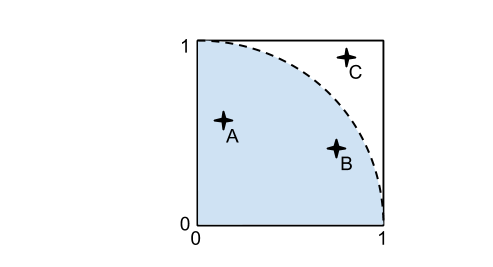
\includegraphics[width=\linewidth]{dartboard}
    \caption{The "dartboard." The computer throws a dart by choosing a random $x$ and $y$ between 0 and 1.  If $x^{2} + y^{2} < 1^{2} $, the dart landed inside the circle.  $A$ and $B$ are darts that landed inside the circle, while $C$ did not.}
    \label{dartboard}
\end{figure}



We tested our framework by running two different MapReduce jobs: a Monte-Carlo approximation of $pi$ and a word frequency count.  
Both jobs were tested under multiple network configurations; we varied the initial size of the network\footnote{The network size changes throughout due to churn, but is unlikely to drastically vary, as the chances of joins and failures are equal.}, the size of the job, and the rate of churn.

Our Monte-Carlo approximation of $\pi$ is largely analogous to having a square with the top-right quarter of a circle going through it (Fig. \ref{dartboard}), and then throwing darts at random locations.  Counting the ratio of darts that land inside the circle to the total number of throws gives us an approximation of $\frac{\pi}{4}$.  The more darts thrown, i.e. the more samples that are taken, the more accurate the approximation\footnote{This is not intended to be a particularly good approximation of $\pi$. Each additional digit of accuracy requires increasing the number of samples taken by an order of magnitude.}

We chose this experiment for a number of reasons. The job is extremely easy to distribute.  This also made it very easy to test scalability. By doubling the amount of samples to collect, we could double the amount of work each node gets without having to store new files on the network.  
Each Map job is defined by the number of throws the node must make and yields a result containing the total number of throws and the number of throws that landed inside the circular section.  Reducing these results is then a matter of adding the respective fields together. 


Our word frequency experiment counts the occurrence of each word in a corpus stored on the Chord network using CFS \cite{CFS}. \textit{We created word frequency counts over a giant list of text from Project Gutenberg.   There are going to be 3 corpus's of text, large enough to show scaling, not so large as to take forever.}   We also varied the block size used for CFS to see what effect that had on computation.  

To perform a word frequency count, the stager obtains the keyfile for the desired corpus and creates a data atom containing the map and reduce functions for each key listed in the keyfile.  Each node receives a data atom for each block they are responsible for and create a word frequency count for their specified blocks.  Those results are reduced by simply combining the word frequency tables. 

%We prove that ChordReduce is scalable and highly fault tolerant, even under high levels of churn and can even benefit from churn under certain circumstances. Specifically, we show it is robust enough to reassign work during runtime in response to nodes entering and leaving the network (Section \textit{ResultsNum}).
\section{Results}

\textit{For $pi$  when we varied x, y happened.  Here's a paragraph an a pretty picture.  Do this a couple more times and you have a results section }\textit{For wordcount, when we varied the blocksize we found this}


\begin{figure}
    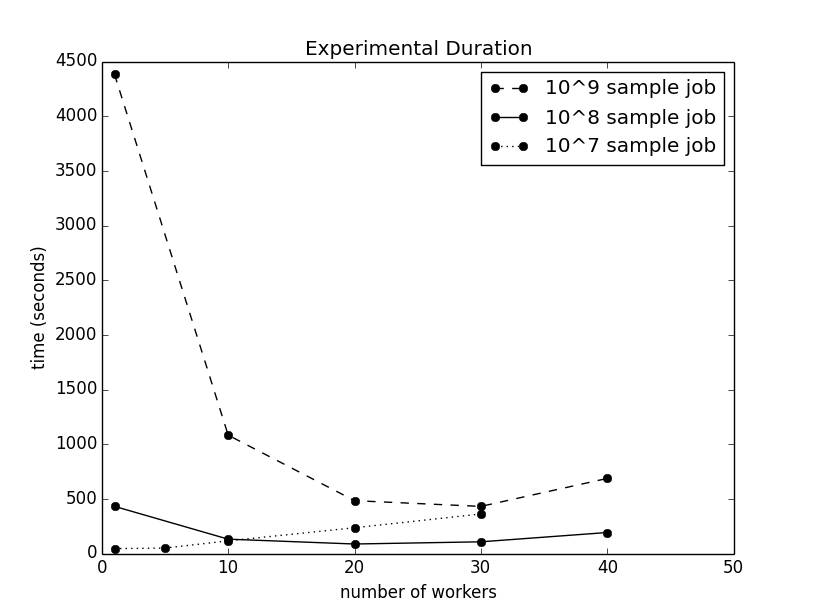
\includegraphics[width=0.5\linewidth]{expTime}
    \caption{For a sufficiently large job, it was almost always preferable to distribute it.  When the job is too small, such as with the $10^{7}$ data set, our runtime is dominated by the overhead.  Our results are what we would expect when overhead grows logarithmically to the number of workers.}
    \label{expTime}
\end{figure}


\begin{figure}
    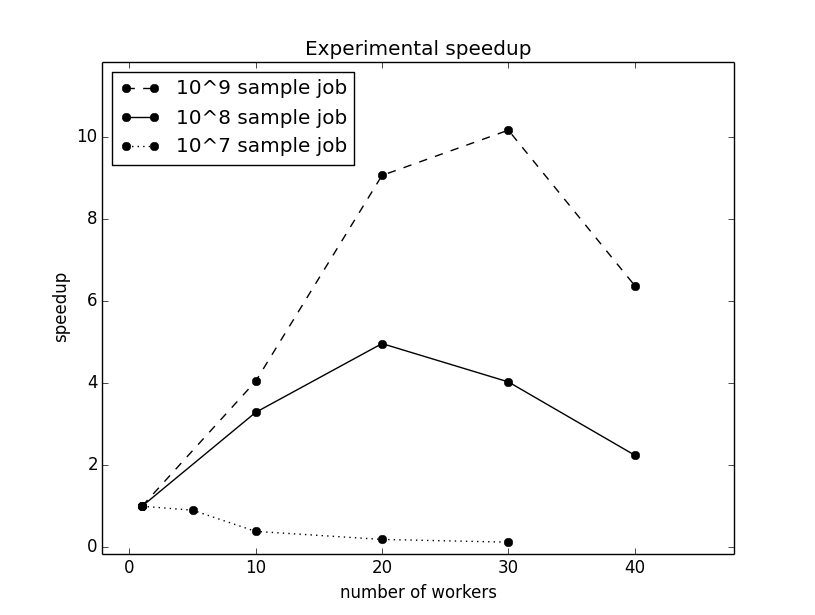
\includegraphics[width=.5\linewidth]{expSpeed}
    \caption{The larger the size of the job, the greater the gains of distributing with ChordReduce.  In addition, the larger the job, the more workers can be added before we start seeing diminishing returns.  This demonstrates that ChordReduce is scalable.}
    \label{expSpeed}
\end{figure}

Fig. \ref{expTime} and Fig. \ref{expSpeed} summarize the experimental results of job duration and speedup.  Our default series was the $10^{8}$ samples series.  On average, it took a single node 431 seconds, or approximately 7 minutes, to generate $10^{8}$ samples.  Generating the same number of samples using ChordReduce over 10, 20, 30, or 40 nodes was always quicker.  The samples were generated fastest when there were 20 workers, with a speedup factor of 4.96, while increasing the number of workers to 30 yielded a speedup of only 4.03.  At 30 nodes, the gains of distributing the work were present, but the cost of overhead ($k \cdot \log_{2}(n)$) had more of an impact.  This effect is more pronounced at 40 workers, with a speedup of 2.25.

Since our data showed that approximating $\pi$ on one node with $10^{8}$ samples took approximately 7 minutes, collecting $10^{9}$ samples on a single node would take 70 minutes at minimum.  Fig. \ref{expSpeed} shows that the $10^{9}$ set gained greater benefit from being distributed than the $10^{8}$ set, with the speedup factor at 20 workers being 9.07 compared to 4.03.  In addition, the gains of distributing work further increased at 30 workers and only began to decay at 40 workers, compared with the $10^{8}$ data set, which began its drop off at 30 workers. This behavior demonstrates that the larger the job being distributed, the greater the gains of distributing the work using ChordReduce.

The $10^{7}$ sample set confirms that the network overhead is logarithmic.  At that size, it is not effective to run the job concurrently and we start seeing overheard acting as the dominant factor in runtime.  This matches the behavior predicted by our equation, $T_{n} = \frac{T_{1}}{n} + k \cdot \log_{2}(n)$. For a small $T_{1}$, $\frac{T_{1}}{n}$  approaches 0 as $n$ gets larger, while $k \cdot \log_{2}(n)$, our overhead, dominates the sample.  The samples from our data set fit this behavior, establishing that our overhead increases logarithmically with the number of workers.


\begin{figure}
    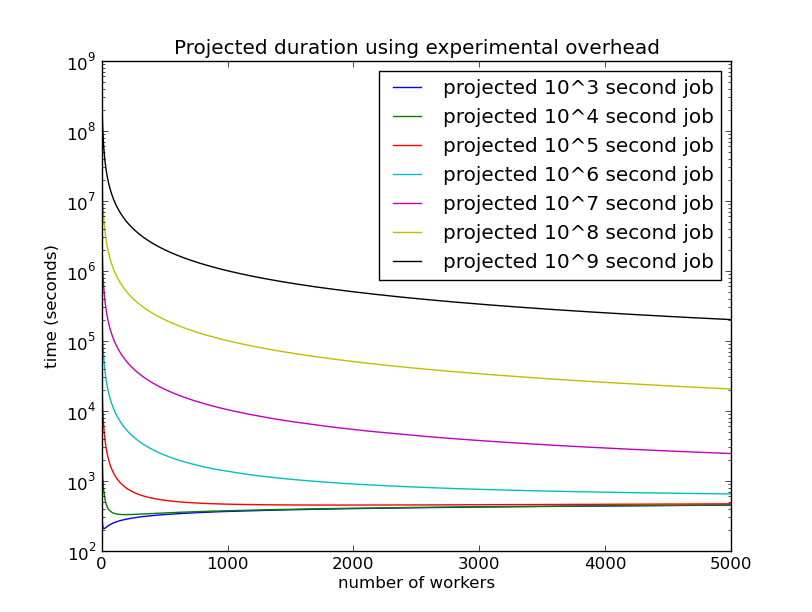
\includegraphics[width=\linewidth]{projTime}
    \caption{The projected runtime using ChordReduce for differently sized jobs.  Each curve projects the expected behavior for job that takes a single worker the specified amount of time.}
    \label{projTime}
\end{figure}

\begin{figure}
    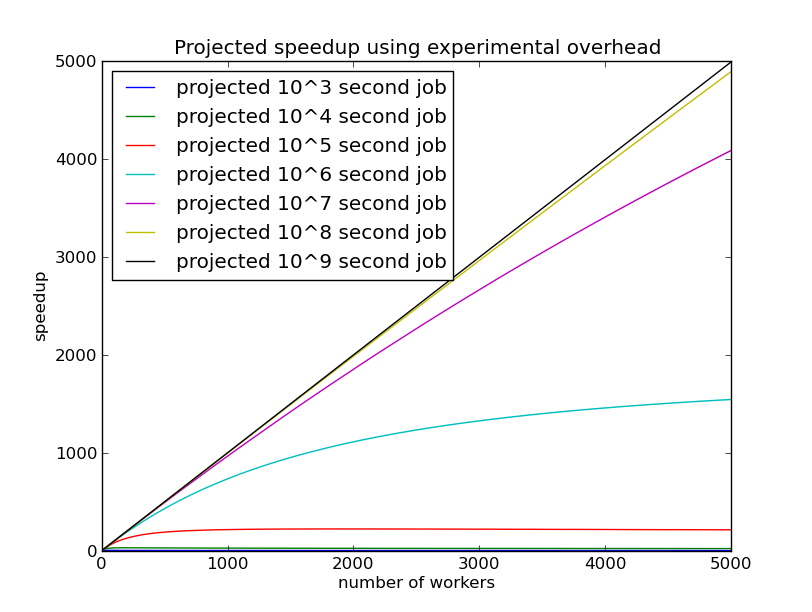
\includegraphics[width=\linewidth]{projSpeed}
    \caption{The projected speedup for different sized jobs. }
    \label{projSpeed}
\end{figure}

Since we have now established that $T_{n} = \frac{T_{1}}{n} + k \cdot \log_{2}(n)$, we can estimate how long a job that takes an arbitrary amount of time to run on a single node would take using ChordReduce.  Our data points indicated that the mean value of $k$ for this problem was 36.5.  Fig. \ref{projTime} shows that for jobs that would take more than $10^{4}$ seconds for single worker to complete, we can expect there would still be benefit to adding an additional worker, even when there are already 5000 workers already in the ring.  Fig. \ref{projSpeed} further emphasizes this. Note that as the jobs become larger, the expected speedup from ChordReduce  approaches linear behavior.


\begin{table}
    \centering
    \begin{tabular}{|r|r|r|} 
        \hline 
        Churn rate per second & Average runtime (s) & Speedup vs 0\% churn\\ \hline{}
        0.8\% & 191.25 & 2.15 \\ \hline
        0.4\% & 329.20 & 1.25 \\ \hline
        0.025\% & 431.86 & 0.95 \\ \hline 
        0.00775\%  & 445.47 & 0.92 \\ \hline 
        0.00250\% & 331.80  &  1.24 \\ \hline 
        0\% & 441.57 & 1.00 \\ \hline
    \end{tabular}
    \caption[Runtime and Speedup versus Churn Rate]{Runtime and Speedup versus Churn Rate} 
    \label{churnSpeed}
\end{table}


Table \ref{churnSpeed} shows the experimental results for different rates of churn. These results show the system  is relatively insensitive to churn.  We started with 40 nodes in the ring and generated $10^{8}$ samples while experiencing different rates of churn, as specified in Table \ref{churnSpeed}.  At the 0.8\% rate of churn, there is a 0.8\% chance each second that any given node will leave the network followed by another node joining the network at a different location. The joining rate and leaving rate being identical is not an unusual assumption to make \cite{marozzo2012p2p} \cite{load}.  

Our testing rates for churn are an order of magnitude higher than the rates used in the P2P-MapReduce simulation  \cite{marozzo2012p2p}.  In their paper, the highest rate of churn was only 0.4\% per minute. Because we were dealing with fewer nodes, we chose larger rates to demonstrate that ChordReduce could effectively handle a high level of churn.  


Our experiments show that for a given problem, ChordReduce can effectively distribute the problem, yielding a substantial speedup.  Furthermore, our results showed that the larger the problem is, the more workers could be added before diminishing returns were incurred.  During runtime, we experienced multiple instances where $plot$ would fail to run and the stager would report socket errors, indicating that it had lost connection with a node in the ring.  Despite this turbulence, every node managed to reestablish connection with each other and report back all the data.  This further demonstrated that we were able to handle the churn in the network.



\section{Related Work}

%We have identified two papers that focus on combining P2P concepts with MapReduce.  Both papers are similar to our research, but differ in crucial ways, as described below.
%\textit{One thing we're pretty sure of is that neither utilizes a blocking scheme like CFS \cite{CFS}, but I'll have to check that}


Marozzo et al. \cite{marozzo2012p2p} investigated the issue of fault tolerance in centralized MapReduce architectures such as Hadoop.  They focused on creating a new P2P based MapReduce architecture built on JXTA \cite{935182} called P2P-MapReduce.  P2P-MapReduce is designed to be more robust at handling node and job failures during execution.

Rather than use a single master node, P2P-MapReduce employs multiple master nodes, each responsible for some job.  If one of those master nodes fails, another will be ready as a backup to take its place and manage the slave nodes assigned to that job.  This avoids the single point of failure that Hadoop is vulnerable to. Failures of the slave nodes are handled by the master node responsible for it.

Experimental results were gathered via simulation and compared P2P-MapReduce to a centralized framework. Their results showed that while P2P-MapReduce generated an order of magnitude more messages than a centralized approach, the difference rapidly began to shrink at higher rates of churn.  When looking at actual amounts of data being passed around the network, the bandwidth required by the centralized approach greatly increased as a function of churn, while the distributed approach again remained relatively static in terms of increased bandwidth usage.  They concluded that P2P-MapReduce would, in general, use more network resources than a centralized approach. However, this was an acceptable cost as the P2P-MapReduce would lose less time from node and job failures \cite{marozzo2012p2p}.


Lee et al.'s work \cite{leemap} draws attention to the fact that a P2P network can be much more than a way to distribute files and demonstrates how to accomplish different tasks using Map and Reduce functions over a P2P network.  Rather than using Chord, Lee et al. used Symphony \cite{symphony}, another DHT protocol with a ring topology.  To run a MapReduce job over the Symphony ring, a node is selected by the user to effectively act as the master.  This ad-hoc master then performs a bounded broadcast over a subsection the ring.  Each node repeats this broadcast over a subsection of that subsection, resulting in a tree with the first node at the top.  

Map tasks are disseminated evenly throughout the tree and their results are reduced on the way back up to the ad-hoc master node.  This allows the ring to disseminate Map and Reduce tasks without the need for a coordinator responsible for distributing these tasks and keeping track of them, unlike Hadoop.  Their experimental results showed that the latency experienced by a centralized configuration is similar to the latency experienced in a completely distributed framework.


%While P2P-MapReduce is decentralized, it still relies on a very definite master/slave hierarchy for organization, computations, and scaling. During simulation, 1\% of the entire network was assigned as master nodes. This means for a simulation of 40000 nodes, 400 were required to organize and coordinate jobs, rendering them unable to do any processing.  In addition, a loosely-consistent  distributed hash table (DHT) such as JXTA can be much slower and fails to maintain the same level of guarantees as an actual DHT, such as Chord \cite{5359174}.   





Both of these papers have promising results and confirm the capability of our own framework and both solely examine P2P networks for the purpose of routing data and organizing the network. ChordReduce uses Chord as a means of efficiently distributing responsibility throughout the network and uses its existing features to add robustness to nodes working on Map and Reduce tasks, in addition to the routing  and organizing capabilities.  Our framework was successfully deployed and tested, operating under high rates of churn without a centralized source for organization. %ChordReduce 

%ChordReduce uses Chord to act as a completely distributed topology for MapReduce, negating the need to assign any explicit roles to nodes or have a scheduler or coordinator.  ChordReduce does not need to assign specific nodes the task of backing up work; nodes backup their tasks using the same process that would be used for any other data being sent around the ring.  Finally, results work their way back to a specified hash address, rather than a specific hash node, eliminating any single point of failure in the network.  These features help prevent a bottleneck from occurring. The result is a simple, distributed, and highly robust architecture for MapReduce.



%The loosely-consistent DHT can be much slower than using an acutal DHT such as Chord .
%Scalability.  A huge issue would be tracking all the nodes and coordinating them. Scalability is handled by mainataining a ratio of masters to slaves 
%Evaluated for low rates of churn.  Such low rates also mean master nodes are barely affected by churn.
%Simulations 
%Our work differs from Marozzo et al.'s in that P2P-MapReduce does not examine using the underlying strengths of a particular P2P protocol or group of protocols, which would have made the architecture simpler.  P2P-MapReduce is decentralized, but still relies on a very definite master/slave hierarchy, while all nodes in ChordReduce are both workers and masters.  We also implemented our MapReduce system rather than simulating the work.

%\subsection{MapReduce using Symphony}
  %However, there are no mechanisms in place to handle churn in the network.  If a node joins during a MapReduce job, it will be unable to contribute any of its resources to the problem. If a node in the bounded broadcast tree fails, or worse the ad-hoc master node fails, the data that node is responsible for is lost. 




\section{Conclusion and Future Work}



We presented ChordReduce, a framework for MapReduce that is completely decentralized, scalable, load balancing, and highly tolerant to churn and node failure at any point in the network. We implemented a fully functional version of ChordReduce and performed detailed experiments to test its performance. These experiments confirmed that ChordReduce is robust and effective. ChordReduce is based on Chord, which is traditionally viewed as a P2P framework for distributing and sharing files.  Instead, we demonstrated that it can also be used as a platform for distributed computation.  Chord provides $\log_{2} n$ connectivity throughout network and has built in mechanisms for handling backup, automatically assigning responsibility, routing, and load balancing. 


Using Chord as the middleware for ChordReduce establishes its effectiveness for distributed and concurrent computation.
The effectiveness of Chord opens up new approaches for tackling other distributed problems, such as supporting databases and machine learning for Big Data, and exascale computations. We intend to further optimize the performance of ChordReduce and extend the middleware to other applications.

%For example, future work could incorporate processes that allow Chord to effectively share and distribute mutable files \cite{IRM} and alter them to perform distributed analysis of mutable data.  These same adjustments can be used to improve the latency of the Chord network with mutable data, which was a major reason why a Chord-based distributed DNS \cite{cox2002serving} was abandoned.  

%While ChordReduce is most efficient when each node is physically close in a cluster, minimizing the impact of latency, this does not exclude the option of tasks being distributed throughout the world.  This setup may be more applicable to a volunteer computing framework, such as Folding@home \cite{folding}.

%Many clusters assume identical or near identical hardware, running an equal amount of nodes, performing an equal amount of work. This is not always a safe assumption to make.  If the hardware used for computations is not equal, then some processors can be left idling when they could be doing more work, while others may be overwhelmed, holding back the rest of the network.

%Adjustments can be easily made on the user's end.  If some hardware can take more work than others, then that system can boot up more instances of nodes locally. Running two nodes locally would mean that approximately twice as much work would assigned to that computer.  Automatically balancing this load is also an avenue for future research.
%Chord could also be used to create a distributed authentication service.



%Our future plans for ChordReduce itself is to recode the library in Java to take advantage of the multiprocessing support, which is limited in Python. 


	

\chapter{A Distributed Greedy Heuristic for Computing Voronoi Tessellations With Applications Towards Peer-to-Peer Networks}
%\author{Double Blind}
\begin{center}
Brendan Benshoof \qquad Andrew Rosen \qquad Anu G. Bourgeois \qquad Robert W. Harrison


Published DPDNS Workshop IPDPS 2015
\end{center}


%  We could use a different config 
% networks are only hpped
% we can do non-euclidean metrics if we have a non-euclidean distance and midpoint definition




\section{Introduction}
\label{sec:intro}

Voronoi diagrams \cite{voronoi} have been used in distributed and  peer-to-peer (P2P) applications for some time. 
They have a wide variety of applications.
Voronoi diagrams can be used as to manage distributed hash tables \cite{virtvoro}, or for in coverage detection for wireless networks \cite{carbunar2004distributed}.
Additionally, Massively Multiplayer Online games (MMOs) can use them to distribute game states and events between players at a large scale \cite{hu2004scalable} \cite{hu2008voronoi} \cite{Backhaus:2007:VAS:1326257.1326266}.

Computing the Voronoi tessellation along with its coprime problem, Delaunay Triangulation, is a well analyzed problem.
There are many algorithms to efficiently compute a Voronoi tessellation given all the points on a plane, such as Fortune's sweep line algorithm \cite{fortune1987sweepline}.
However, many network applications are distributed and many of the algorithms to compute Voronoi tessellations are unsuited to a distributed environment.

In addition, complications occurs when points are located in spaces with more than two dimensions.
Computing the Voronoi tessellation of $n$ points in a space with $d$ dimensions takes $O(n^{\frac{2d-1}{d}})$ time \cite{watson1981computing}.
Distributed computations often have to resort to costly Monte-Carlo calculations \cite{raynet} in order to handle more than two dimensions.

%We take advantage of the fact that distributed applications are fault-tolerant to accommodate changes in network topology.
%This is especially true for P2P environments.
Rather than exactly solving the Voronoi tessellation, we instead present a fast and accurate heuristic to approximate each of the regions of a Voronoi tessellation.
This enables fast and efficient formation of P2P networks, where nodes are the Voronoi generators of those region.
A P2P network built using this heuristic would be able to take advantage of its available fault-tolerant architecture to route along any inaccuracies that arise.
Our paper presents the following contributions:
\begin{itemize}
	\item We present our Distributed Greedy Voronoi Heuristic (DGVH). 
	The DGVH is a fast, distributed, and highly accurate method, whereby nodes calculate their individual regions described by a Voronoi tessellation using the positions of nearby nodes.
	DGVH can work in an arbitrary number of dimensions and can handle non-euclidean distance metrics.
    Our heuristic can also handle toroidal spaces.
	In addition, DGVH can accommodate the calculation of nodes moving their positions and adjust their region accordingly, while still maintaining a high degree of accuracy (Section \ref{sec:dgvh}).
    Even where small inaccuracies exist, DVGH will create a fully connected graph.
	\item We discuss how P2P networks and distributed applications can use DGVH (Section \ref{sec:applications}).
	In particular, we show how we can use DGVH to build a distributed hash table with embedded minimal latency.
	\item We present simulations demonstrating DGVH's efficacy in quickly converging to the correct Voronoi tessellation.
    We simulated our heuristic in networks ranging from size 500 nodes to 10000 nodes.
	Our simulations show that a distributed network running DGVH accurately determines the region a randomly chosen point falls in 90\% of the time within 20 cycles and converges near 100\% accuracy by cycle 30 (Section \ref{sec:experiments}).
	\item We present the related work we have built upon to create our heuristic and what improvements we made with DGVH (Section \ref{sec:related}).
\end{itemize}


\section{Distributed Greedy Voronoi Heuristic}
\label{sec:dgvh}


A Voronoi tessellation is the partition of a space into cells or regions along a set of objects $O$, such that all the points in a particular region are closer to one object than any other object.  
We refer to the region owned by an object as that object's Voronoi region.
Objects which are used to create the regions are called Voronoi generators.
In network applications that use Voronoi tessellations, nodes in the network act as the Voronoi generators.

The Voronoi tessellation and Delaunay triangulation are dual problems, as an edge between two objects in a Delaunay triangulation exists if and only if those object's Voronoi regions border each other.  
This means that solving either problem will yield the solution to both.   
An example Voronoi diagram is shown in Figure \ref{voro-ex}.
For additional information, Aurenhammer \cite{voronoi} provides a formal and extremely thorough description of Voronoi tessellations, as well as their applications.


\begin{figure}
	\centering
	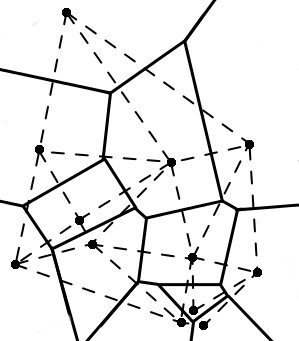
\includegraphics[width=0.75\linewidth]{voronoi}
	\caption{An example Voronoi diagram for objects on a 2-dimensional space.  The black lines correspond to the borders of the Voronoi region, while the dashed lines correspond to the edges of the Delaunay Triangulation.}
	\label{voro-ex}
\end{figure}



\subsection{Our Heuristic}




%take for granted that it requires a fast and efficient way to compute Voronoi tessilations in an arbitrary number of dimensions.
%The Distributed Greedy Voronoi Heuristic (DGVH) is a fast method for nodes to select peers from their Deluanay Triangulation (Algorithm \ref{DGVH}).
The Distributed Greedy Voronoi Heuristic (DGVH) is a fast method for nodes to define their individual Voronoi region (Algorithm \ref{alg:dgvh}). 
This is done by selecting the nearby nodes that would correspond to the points connected to it by a Delaunay triangulation.
The rationale for this heuristic is that, in the majority of cases, the midpoint between two nodes falls on the common boundary of their Voronoi regions.

%In addition, nodes should only have to compute their own Voronoi region, and possibly estimate those of its neighbors. 
%Anything else is a waste of processing power.



\begin{figure} % make smaller
\caption{Distributed Greedy Voronoi Heuristic}
\label{alg:dgvh}
\begin{algorithmic}[1]  % the numberis how many lines
	 \State Given node $n$ and its list of $candidates$.
   	 \State Given the minimum $table\_size$
    \State $short\_peers \leftarrow$ empty set that will contain $n$'s one-hop peers
	 \State $long\_peers \leftarrow$ empty set that will contain $n$'s two-hop peers    
    \State Sort $candidates$ in ascending order by each node's distance to $n$
    \State Remove the first member of $candidates$ and add it to $short\_peers$
    \For{$c$ in $candidates$}
        \If{Any node in $short\_peers$ is closer to $c$ than $n$}
        	\State Reject $c$ as a peer
        \Else
        	\State Remove $c$ from $candidates$
        	\State Add $c$ to $short\_peers$
        \EndIf
    \EndFor
    \While{ $|short\_peers| < table\_size$ AND $|candidates| >0$ }
    	\State Remove the first entry $c$ from $candidates$
    	\State Add $c$ to $short\_peers$
    \EndWhile
    	\State Add $candidates$ to the set of $long\_peers$	
    	\If{$|long\_peers| > table\_size^2$}
        		\State $long\_peers \leftarrow$ random subset of $long\_peers$ of size $table\_size^2$
      \EndIf
\end{algorithmic}
\end{figure}


During each cycle, nodes exchange their peer lists with a current neighbor and then recalculate their neighbors.  
A node combines their neighbor's peer list with its own to create a list of candidate neighbors.
This combined list is sorted from closest to furthest.
A new peer list is then created starting with the closest candidate.
The node then examines each of the remaining candidates in the sorted list and calculates the midpoint between the node and the candidate.
If any of the nodes in the new peer list are closer to the midpoint than the candidate, the candidate is set aside.  
Otherwise the candidate is added to the new peer list.







% \subsubsection*{The following paragraphs may need reordering}


DGVH never actually solves for the actual polytopes that describe a node's Voronoi region.
This is unnecessary and prohibitively expensive \cite{raynet}.
Rather, once the heuristic has been run, nodes can determine whether a given point would fall in its region.

Nodes do this by calculating the distance of the given point to itself and other nodes it knows about.
The point falls into a particular node's Voronoi region if it is the node to which it has the shortest distance.
This process continues recursively until a node determines that itself to be the closest node to the point.
Thus, a node defines its Voronoi region by keeping a list of the peers that bound it.



%maybe move this paragraph to analysis
This heuristic has the benefit of being fast and scalable into any geometric space where a distance function and midpoint can be defined.
The distance metric used for this paper is the minimum distance in a multidimensional unit toroidal space.
Where $\vec{a}$ and $\vec{b}$ are locations in a $d$-dimensional unit toroidal space:
\[ distance = \sqrt{\sum\limits_{i\in d} (\min(|\vec{a}_i-\vec{b}_i|, 1-|\vec{a}_i-\vec{b}_i|))^2}\]
Whether or not distance corresponds to actual physical distance or some virtual distance on an overlay depends on the application.

%In two-dimensional spaces, there is quick hack to achieve 100\% accuracy distributed.

Our heuristic can be overaggressive in removing candidate nodes.
For example, if a node is located between two other nodes, such that their midpoint does not fall upon the shared face of their Voronoi regions, then this heuristic will not link the blocked peers.
This is demonstrated in Figure \ref{occ-ex}.
\begin{figure}
	\centering
	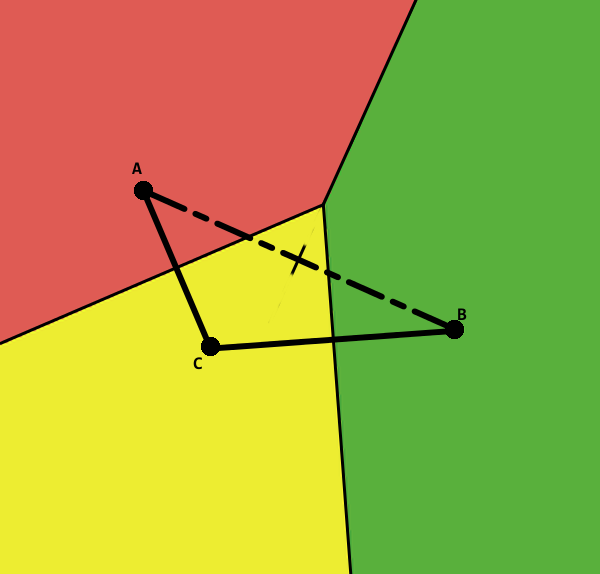
\includegraphics[width=\linewidth]{occlusion}
	\caption{The edge between $A$ and $B$ is not detected by DGVH, as node $C$ is closer to the midpoint than $B$ is.  This is mitigated by peer management polices.}  %Add labels a b c and reference the node labels in text
	\label{occ-ex}
\end{figure}
Our algorithm handles these cases via our method of peer management (Section \ref{sec:manage}).
%Overaggressive pruning by a single nodes is handled by neighboring nodes. 
%So long as a single node determines that an edge exists, it will advertise that edge's existence.






\subsection{Peer Management}
\label{sec:manage}
Nodes running the heuristic maintain two peer lists: \textit{Short Peers} and \textit{Long Peers}.
This is done to mitigate the error induced by DGVH and provide robustness against churn\footnote{The disruption caused to an overlay network by the continuous joining, leaving, and failing of nodes.} in a distributed system.

\textit{Short Peers} are the set of peers DGVH judged to have Voronoi regions adjacent to the node's own. 
Using a lower bound on the length of \textit{Short Peers} corrects for errors in the approximation as it forces nodes to include peers that would otherwise be omitted. 
Previous work by Beaumont \textit{et al}.\ \cite{raynet} has found a useful lower bound on short peers to be $3d + 1$.
Should the number of short peers generated by DGVH be less than the lower bound, the nearest peers not already included in \textit{Short Peers} are added to it, until \textit{Short Peers} is of sufficient size.
%Members of \textit{Short Peers} are analogous to the predecessors/successors in other DHTs.



There is no upper bound to the number of short peers a node can have.
This means in contrived cases, such as a single node surrounded by other nodes forming a hypersphere, this number can grow quite high.
Bern \textit{et al.\ }\cite{bern1991expected} found that the expected maximum degree of a vertex in a Delaunay Triangulation is
$$\Theta(\frac{\log n}{\log \log n} )$$ 
where $n$ is the number of nodes in the Delaunay Triangulation. 
This bound applies to a Delaunay Triangulation in any number of dimensions.
Thus, the maximum expected size of \textit{Short Peers} is bounded by $\Theta(\frac{\log n}{\log \log n} )$, which is a highly desirable number in many distributed systems \cite{chord} \cite{kademlia}.



\textit{Long Peers} is the list of two-hop neighbors of the node.
When a node learns about potential neighbors, but are not included in the short peer list, they may be included in the long peer list.  
\textit{Long Peers} has a maximum size of $(3d+1)^2$, although this size can be tweaked to the user's needs.  
For example, if \textit{Short Peers} has a minimum size of 8, then \textit{Long Peers} has a maximum of 64 entries.  
We recommend that members of \textit{Long Peers} are not actively probed during maintenance to minimize the cost of maintenance.
A maximum size is necessary, as leaving it unbounded would result in a node eventually keeping track of all the nodes in the network, which would be counter to the design of a distributed and scalable system.

%We next discuss how nodes learn about short and long peers.
How nodes learn about peers is up to the application.
We experimented using a gossip protocol, whereby a node selects peers from \textit{Short Peers} at random to ``gossip'' with.
When two nodes gossip with each other, they exchange their \textit{Short Peers} with each other.
The node combines the lists of short peers\footnote{Nodes remove themselves and repetitions from the candidates they receive.} and uses DGVH to determine which of these candidates correspond to its neighbors along the Delaunay Triangulation.
The candidates determined not to be short peers become long peers.  
If the resulting number of long peers exceeds the maximum size of \textit{Long Peers}, a random subset of the maximum size is kept.

The formal algorithm for this process is described in Algorithm~\ref{alg:gossip}.
This maintenance through gossip process is very similar to the gossip protocol used in Beaumont et al.'s RayNet \cite{raynet}.


\begin{figure}
\caption{Gossiping}
\label{alg:gossip}
\begin{algorithmic}[1]  % the number is how many 
	\State Node $n$ initiates the gossip.
	\State $neighbor \leftarrow$ random node from $n.short\_peers$
   \State $n\_candidates \leftarrow n.short\_peers \cup n.long\_peers \cup neighbor.short\_peers$
   \State $neighbor\_candidates \leftarrow neighbor.short\_peers \cup neighbor.long\_peers \cup n.short\_peers$.  
   \State $n$ and $neighbor$ each run Distributed Greedy Voronoi Heuristic using their respective $candidates$
\end{algorithmic} 
\end{figure}






\subsection{Algorithm Analysis}

DVGH is very efficient in terms of both space and time.
Suppose a node $n$ is creating its short peer list from $k$ candidates in an overlay network of $N$ nodes. 
The candidates must be sorted, which takes $O(k\cdot\lg(k))$ operations.  
Node $n$ must then compute the midpoint between itself and each of the $k$ candidates.  
Node $n$ then compares distances to the midpoints between itself and all the candidates.  
This results in a cost of 

\[ k\cdot\lg(k) + k \text{ midpoints}  + k^{2} \text{ distances} \]


Since $k$ is  bounded by $\Theta(\frac{\log N}{\log \log N} )$ \cite{bern1991expected} (the expected maximum degree of a node), we can translate the above to

\[O(\frac{\log^{2} N}{\log^{2} \log N} )\]

In the vast majority of cases, the number of peers is equal to the minimum size of \textit{Short Peers}. 
This yields $k=(3d+1)^{2}+3d+1$ in the expected case, where the lower bound and expected complexities are $\Omega(1)$.

Previous work \cite{raynet} claims constant time approximation. 
The reality is that Raynet's leading constant is in the order of thousands. % as Monte-Carlo samples.  
Our algorithm has a greater asymptotic worst case cost, but for all current realistic network sizes it will be more time efficient then RayNet's approximation.





\section{Applications}
\label{sec:applications}

As we previously discussed in Section \ref{sec:intro}, Voronoi tessellation have many applications for distributed systems \cite{carbunar2004distributed} \cite{hu2004scalable} \cite{hu2008voronoi} \cite{Backhaus:2007:VAS:1326257.1326266}.
We focus our discussion on the two extremes of applications: DHTs, which work with overlay networks, and wireless networks, which need to take literal physical constraints into account.




\subsection{Distributed Hash Tables and Voronoi tessellation}
Arguably all Distributed Hash Tables (DHTs) are built on the concept of Voronoi tessellation.
In all DHTs, a node is responsible for all points in the overlay to which it is the ``closest'' node.
Nodes are assigned a key as their location in some keyspace, based on the hash of certain attributes.
Normally, this is just the hash of the IP address (and possibly the port) of the node \cite{chord} \cite{kademlia} \cite{can} \cite{pastry}, but other metrics such as geographic location can be used as well \cite{ratnasamy2002ght}.

These DHTs have carefully chosen metric spaces such that these regions are very simple to calculate.
For example, Chord \cite{chord} and similar ring-based DHTs \cite{manku2003symphony} utilize a unidirectional, one-dimensional ring as their metric space, such that the region for which a node is responsible is the region between itself and its predecessor.

Using a Voronoi tessellation in a DHT generalizes this design. 
Nodes are Voronoi generators at a position based on their hashed keys.
These nodes are responsible for any key that falls within its generated Voronoi region.

Messages get routed along links to neighboring nodes. 
This would take $O(n)$ hops in one dimension.
In multiple dimensions, our routing algorithm (Algorithm \ref{alg:lookup}) is extremely similar to the one used in Ratnasamy et al.'s Content Addressable Network (CAN) \cite{can}, which would be $O(n^{\frac{1}{d}})$ hops.
\begin{figure}
	\caption{Lookup in a Voronoi-based DHT}
	\label{alg:lookup}
	\begin{algorithmic}[1] 
		\State Given node $n$
		\State Given $m$ is a message addressed for $loc$
		\State $potential\_dests \leftarrow n \cup n.short\_peers \cup n.long\_peers$
		\State $c \leftarrow $ node in $ potential\_dests$ with shortest distance to $loc$
		\If{$c$ == $n$}
		\Return $n$
		\Else
		\Return $c.lookup(loc)$
		\EndIf
	\end{algorithmic}
\end{figure}

DGVH can be used in a DHT to quickly and scalably construct both the Voronoi tessellation and links to peers.
%TODO Numbers to back up needed?
In addition, gossip-based peer management policies are extremely efficient in proactively handling node joins and failures.
The act of joining informs other nodes of the joiner's existence.
This can be done by the joiner contacting each peer in the peer lists of the node previously responsible for the joiner's location.

Node failures can be handled without much effort.
When a node attempts to route to or gossip with a node and discovers it no longer exists, it should remove the node from its peer lists and inform all of the nodes it knows to do the same.
Since routing is how a node would make a decision on whether a point belongs to a particular Voronoi region, failed nodes don't have any impact on the network's accuracy.


Because the algorithm is defined in terms of midpoint and distance functions, it is not bound to any particular topology or metric space.
Our heuristic can be used to create a DHT that uses any arbitrary coordinate system which defines a midpoint and distance definition.

For example, we could use latency as one of these metrics by using it to approximate node locations in the network.
This would allow messages to be routed along minimum latency paths, rather than along minimal hop paths.
We intend to model this using a distributed spring model.


\subsection{Wireless Coverage}
C\u{a}rbunar et al.\ \cite{carbunar2004distributed} demonstrated how Voronoi tessellations could be used to solve the \textit{coverage-boundary} problem in wireless ad-hoc networks.
The coverage-boundary problem asks which nodes are on the physical edge of the network.
This knowledge provides useful information to networks.
For example, ad-hoc networks operating in no infrastructure or have been set up temporarily can use this knowledge to define the reach of the network's coverage.

The authors showed how a Voronoi tessellation using the nodes as Voronoi generators could solve the coverage-boundary problem.
They proved that the node's Voronoi region was not completely covered by the node's sensing radius if and only if the node was on the network's boundary \cite{carbunar2004distributed}.

%Move lower?
Chen et al.\ \cite{chen2008voronoi} extended this property for sleep scheduling in wireless sensor networks.
A node is allowed to go to sleep and conserve power so long as the area it is detecting can be covered by other nodes.
Using Voronoi tessellations, a node knows it can conserve power and not affect the network if and only if it is not on the boundary of the network and its Voronoi vertices\footnote{Voronoi vertices are the points at which the edges of 3 or more Voronoi cells converge.} are covered by other nodes.


C\u{a}rbunar et al.'s algorithm relies on a centralized computation for Voronoi tessellation, as the distributed computation they examined only relied on forming the Delaunay triangulation between nodes within a certain radius, nor could it handle moving nodes.
DGVH is not limited to handling nodes within a specified radius, since the peer management spreads information about nodes by gossiping. %like old yiddish women.
In addition, so long as a node moving to a new location is treated as an entirely new node by the rest of the network, DGVH can handle moving nodes.\footnote{A specific node and a specific location must be bound together into a single identity.
This means when a node tries to route to a node that has moved using the node's previous location, it should fail, as though that specific node no longer exists.  
Failure to do this would cause a node to incorrectly determines what falls within its Voronoi region.}


\section{Experiments}
\label{sec:experiments}


We implemented two sets of experiments for DGVH.
The first compares the Voronoi tessellations created by DGVH to an actual Voronoi tessellation.
Our second set of experiments demonstrates that any errors computed by DGVH are negligible when building distributed and fault-tolerant systems.

\subsection{Experiment 1: Voronoi Accuracy}

To test the accuracy of our heuristic, we have generated the graphs produced DGVH and a Delaunay triangulation generated by the Triangle \cite{shewchuk96b} library.
We tested in 2-dimensional euclidean space and measured the number of edges in the graph generated by DGVH that differ from the graph generated by a Delaunay Triangulation.
We tested networks of 100, 500, 1000, 2000, and 5000 nodes and found that the graphs by DGVH differed from the graph generated Delaunay triangulation by approximately 1 edge per node.
Our results are summarized in Figure \ref{exp_0}.


\begin{figure}
	\centering
	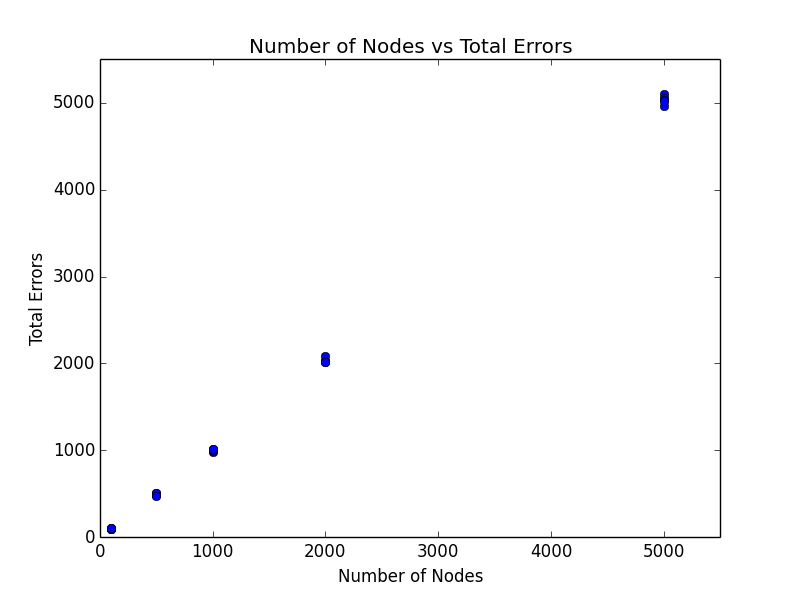
\includegraphics[width=0.75\linewidth]{error_rate}
	\caption{As the size of the graph increases, we see approximately 1 error per node.}
	\label{exp_0}
\end{figure}







\subsection{Experiment 2: P2P Convergence and Routing}
Our second set of experiments examines how DGVH could be used to create a DHT and how well it would perform in this task.
Our simulation demonstrates how DGVH  can be used to create a stable overlay from a chaotic starting topology after a sufficient number of gossip cycles.  
We do this by showing that the rate of successful lookups approaches 1.0.
We compare these results to RayNet \cite{raynet}, which proposed that a random $k$-connected graph would be a good, challenging starting configuration for demonstrating convergence of a DHT to a stable network topology.

During the first two cycles of the simulation, each node bootstraps its short peer list by appending 10 nodes, selected uniformly at random from the entire network.
In each cycle, the nodes gossip (Algorithm \ref{alg:gossip}) and run DGVH using the new information.
We then calculate the hit rate of successful lookups by simulating 2000 lookups from random nodes to random locations, as described in Algorithm \ref{routesim}.
A lookup is successful when the network correctly determines which Voronoi region contains a randomly selected point.


Our experimental variables for this simulation were the number of nodes in the DGVH generated overlay and the number of dimensions.  
We tested network sizes of 500, 1000, 2000, 5000, and 10000 nodes each in 2, 3, 4, and 5 dimensions.
The hit rate at each cycle is $\frac{hits}{2000}$, where $hits$ are the number of successful lookups.




\begin{figure}
	\caption{Routing Simulation Sample}
	\label{routesim}
	\begin{algorithmic}[1]  % the number is how many 
		\State $start \leftarrow$ random node
		\State $dest \leftarrow$ random set of coordinates
		\State $ans \leftarrow$ node closest to $dest$
		\If{$ans == start.lookup(dest)$}
		\State increment $hits$
		\EndIf
	\end{algorithmic} 
\end{figure}


%In order to show that leaving the size of the short peer list unbounded is not detrimental to the memory costs of nodes, we also kept track of the size of the short peer list at each cycle. 

%\subsection{Convergence Simulation Results}
Our results are shown in Figures \ref{conv2}, \ref{conv3}, \ref{conv4}, and \ref{conv5} for each dimension.
Our graphs show that the created overlay quickly constructs itself from a random configuration and that our hit rate reached 90\% by cycle 20, regardless of dimension.
Lookups consistently approached a hit rate of 100\% by cycle 30. 
In comparison, RayNet's routing converged to a perfect hit rate at around cycle 30 to 35 \cite{raynet}.
As the network size and number of dimensions each increase, convergence slows, but not to a significant degree.

\begin{figure*}
	\label{fig:conv}
	\centering 
	\begin{tabular}{cc}
		
		\begin{subfigure}{\columnwidth}
			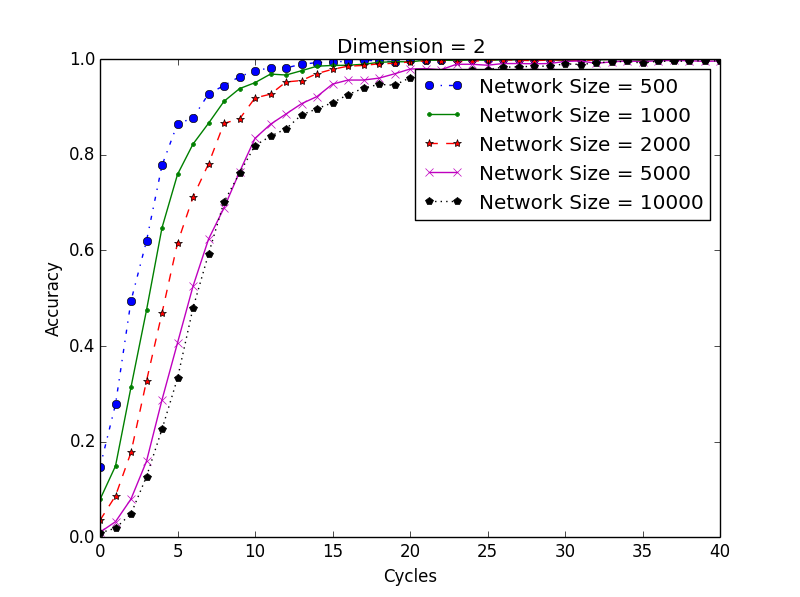
\includegraphics[width=\columnwidth]{conv_d2}
			\caption{This plot shows the accuracy rate of lookups on a 2-dimensional network as it self-organizes.}
			\label{conv2}
		\end{subfigure} &
		
		\begin{subfigure}{\columnwidth}
			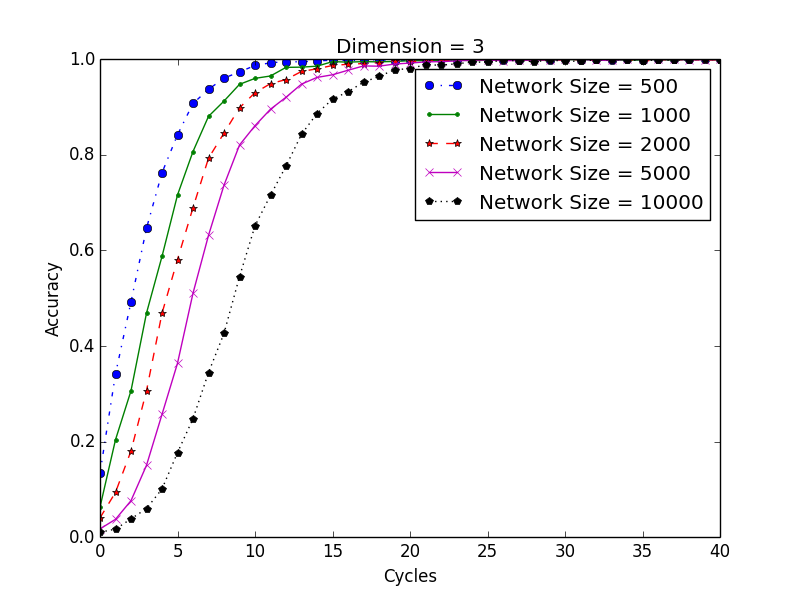
\includegraphics[width=\columnwidth]{conv_d3}
			\caption{This plot shows the accuracy rate of lookups on a 3-dimensional network as it self-organizes.}
			\label{conv3}
		\end{subfigure} \\
		
		\begin{subfigure}{\columnwidth}
			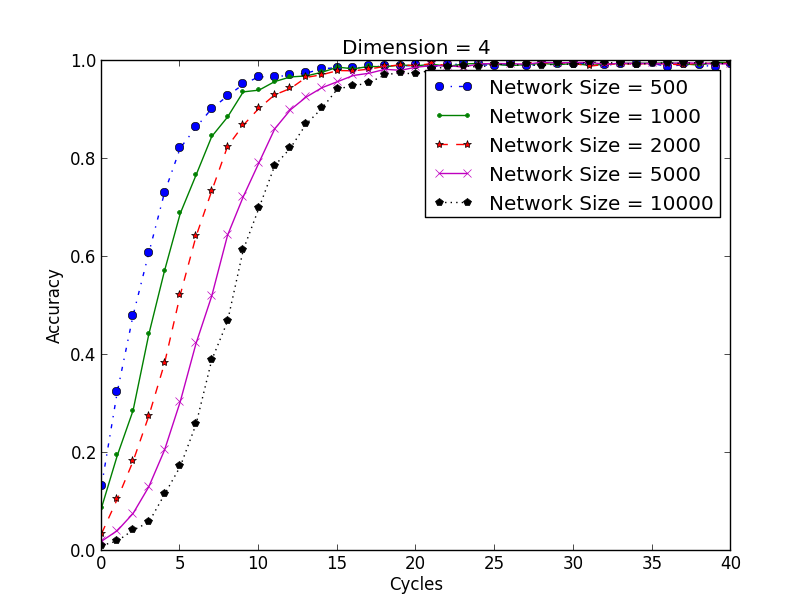
\includegraphics[width=\linewidth]{conv_d4}
			\caption{This plot shows the accuracy rate of lookups on a 4-dimensional network as it self-organizes.}
			\label{conv4}
		\end{subfigure} &
		
		
		\begin{subfigure}{\columnwidth}
			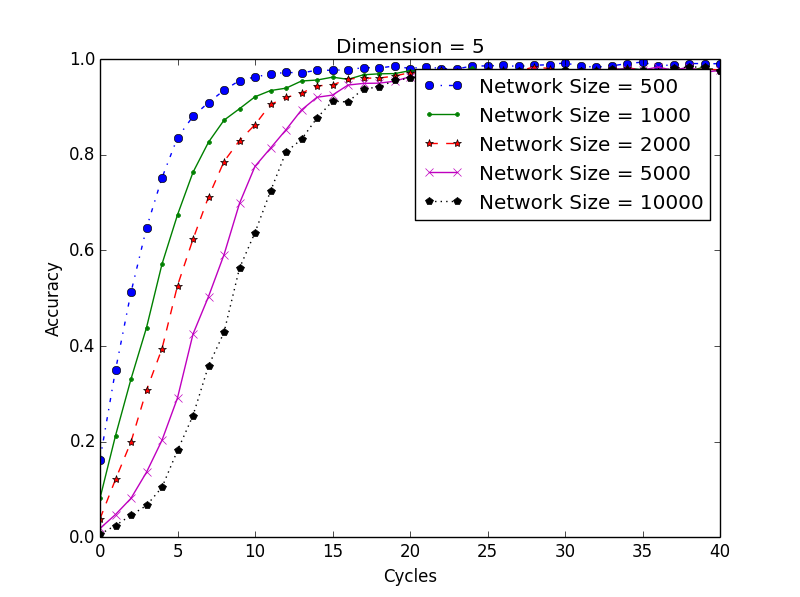
\includegraphics[width=\linewidth]{conv_d5}
			\caption{This plot shows the accuracy rate of lookups on a 5-dimensional network as it self-organizes.}
			\label{conv5}
		\end{subfigure}
		
	\end{tabular}
	\caption{These figures show that, starting from a randomized network, DGVH forms a stable and consistent network topology.
		The Y axis shows the success rate of lookups and the X axis show the number of gossips that have occurred.
		Each point shows the fraction of 2000 lookups that successfully found the correct destination.}
	
\end{figure*}

\begin{table}
\centering
\begin{tabular}{|r|r|r|r|}
\hline
Network Size & Dimensions & avg degree & max degree\\ \hline
500   & 2 & 7.004 & 8 \\ \hline
1000  & 2 & 7.001 & 8 \\ \hline
2000  & 2 & 7.0015 & 8 \\ \hline
5000  & 2 & 7.0364 & 66 \\ \hline
10000 & 2 & 8.0151 & 81\\ \hline  % the heck?
500   & 3 & 10.364 & 16 \\ \hline
1000  & 3 & 10.321 & 15 \\ \hline
2000  & 3 & 10.272 & 16 \\ \hline
5000  & 3 & 10.3264 & 18 \\ \hline
10000 & 3 & 9.1233 & 19 \\ \hline
500   & 4 & x & x \\ \hline
1000  & 4 & x & x \\ \hline
2000  & 4 & x & x \\ \hline
5000  & 4 & x & x \\ \hline
10000 & 4 & x & x \\ \hline
500   & 5 & x & x \\ \hline
1000  & 5 & x & x \\ \hline
2000  & 5 & x & x \\ \hline
5000  & 5 & x & x \\ \hline
10000 & 5 & x & x \\ \hline
\end{tabular}
\caption{Information about the size short peer lists, denoted degree here, at the last cycle of the convergence simulation.  For each pair of network size and dimension, we report the average degree in the network, as well as the largest.}
\label{tab:convtable}
\end{table}


\section{Related Work}
\label{sec:related}
%check table size consistancy 
While there has been previous work on applying Voronoi regions to DHTs and peer-to-peer (P2P) applications, we have found no prior work on how to perform embedding of an inter-node latency graph.   

Backhaus et al.'s  VAST \cite{Backhaus:2007:VAS:1326257.1326266} is a Voronoi-based P2P protocol designed for handling event messages in a massively multiplayer online video game.  
Each node finds its neighbors by constructing a Voronoi diagram using Fortune's sweepline algorithm \cite{fortune1987sweepline}.  
VAST demonstrated that Voronoi diagrams could be used as the backbone to large-scale applications, although their work focused specifically on using 2-dimensional Voronoi diagrams.

The two DHT protocols developed by Beumont et al., VoroNet \cite{voronet} and RayNet \cite{raynet} are two-dimension DHTs that we intend to extend using our technique.
VoroNet is based off Kleinberg's small world model \cite{kleinberg2000navigation} and achieves polylogarithmic lookup time.  
Each node in VoroNet solves its Voronoi region to determine its neighbors and also maintains a link to a randomly chosen distant node.
VoroNet focused specifically on the two-dimensional Voronoi computations and the techniques used would be too expensive in higher dimensions and were not resilient to churn  \cite{raynet}.

RayNet \cite{raynet} was based on the work done on VoroNet and used a heuristic to calculate Voronoi tessilations.  
Like our DGVH, RayNet's heuristic does not solve for Voronoi regions, as that is prohibitively expensive.  
RayNet uses a Monte-Carlo method to approximate the volume of a node's Voronoi region in constant time.  
While effective at estimating the Voronoi region,  the volume-based Monte-Carlo approximation is expensive and requires multiple samples. 
This gives the runtime of RayNet's heuristic an enormous leading constant.
RayNet does mention the idea of mapping attributes to each axis, but how this can be exploited is left as future work.




%Unlike ACE, we handle unbounded simultaneous join and leave operations.



\section{Conclusion and Future Work}
\label{sec:conclusion}


Voronoi tessellations have a wide potential for applications in ad-hoc networks, massively multiplayer games, P2P, and distributed networks. 
However, centralized algorithms for Voronoi tessellation and Delaunay triangulation are not applicable to decentralized systems.
In addition, solving Voronoi tessellations in more than 2 dimensions is computationally expensive.

We created a distributed heuristic for Voronoi tessellations in an arbitrary number of dimensions.
Our heuristic is fast and scalable, with a expected memory cost of $(3d+1)^{2}+3d+1$ and expected maximum runtime of O$(\frac{\log^{2} N}{\log^{2} \log N} )$.

We ran two sets of experiments to demonstrate DGVH's effectiveness.
Our first set of experiments demonstrated that our heuristic is reasonably accurate  and our second set demonstrates that reasonably accurate is sufficient to build a P2P network which can route accurately.


Our next step is to create a formal protocol and implementation for a Voronoi tessellation-based distributed hash table using DGVH.  
We can use this DHT to choose certain metrics we want to measure, such as latency, or trust, and embed that information as part of a node's identity.
By creating an appropriate distance measurement, we can route along some path that minimizes or maximizes the desired metric.
Rather than create an overlay that minimizes hops, we can have our overlay minimize latency, which is the actual goal of most routing algorithms.


%Another venue for exploration is application of caching and replication strategies to a functional distributed file system running on top of VHash.  Such extensions seek to improve upon existing work done on file replication and caching schemes \cite{shen2010irm}.

	\chapter{UrDHT: A Unified Model for Distributed Hash Tables}


\begin{center}
Andrew Rosen \qquad Brendan Benshoof \qquad Robert W. Harrison \qquad Anu G. Bourgeois

Under consideration by ICPP 2016
\end{center}



\section{Introduction}
%Distributed Hash Tables (DHT) have been extensively researched for the past decade.
%Many different DHT protocols have developed over the years.
%What is a DHT
% Mention the DHT API
%Despite this, no one has created a cohesive formal specification for building a DHT. % or something


%UrDHT is our specification and implementation of an abstract DHT.



We present UrDHT, an abstract model of a distributed hash table (DHT). %that solves a number of problems.
It is a unified and cohesive model for creating DHTs and P2P applications based on DHTs.
%UrDHT also provides a single network for bootstrapping distributed applications.
%Third, we show that using the abstraction features of UrDHT, we can embed latency into the DHT's overlay.
%
%\subsubsection{Abstraction}

Distributed Hash Tables have been the catalyst for the creation of many P2P applications.
Among these are Redis \cite{redis}, Freenet \cite{freenet}, and, most notably, BitTorrent \cite{bittorrent}. 
All DHTs use functionally similar protocols to perform lookup, storage, and retrieval operations.
Despite this, no one has created a cohesive formal DHT specification.

Our primary motivation for this project was to create an abstracted model for Distributed Hash Tables based on observations we made during previous research \cite{dgvh}.
We found that all DHTs can cleanly be mapped to the primal-dual problems of Voronoi Tessellation and Delaunay Triangulation.

%TODO Match vocabulary
UrDHT builds its topology directly upon this insight.
It uses a greedy distributed heuristic for approximating Delaunay Triangulations.
We found that we could reproduce the topology of different DHTs by defining a selection heuristic and rejection algorithm for the geometry the DHT.
For every DHT we implemented, our greedy approximation of Delaunay Triangulation produced a stable DHT, regardless of the geometry.  
This works in non-Euclidean geometries such as XOR (Kademlia) or even a hyperbolic geometry represented by a Poincar\`{e} disc.

The end result is not only do we have an abstract model of DHTs, we have a simple framework that developers can use to quickly create new distributed applications.
This simple framework allows generation of internally consistent implementations of different DHTs that can have their performance rigorously compared.  %we can now test DHTs against each other fairly



%\subsubsection{Bootstrapping}
%Another poorly addressed issue within DHTs and DHT-based P2P applications we wish to tackle with UrDHT is the what we have termed the \textit{bootstrapping problem}.
%Simply put, a node can only join the network if it knows another node that is already a member of the network it is trying to join.
%%Current distributed systems suffer from fragmentation, high overhead, and an inability to scale due to difficulty of adoption.
%
%The way this generally works is by having a potential user manually look up at a centralized source, such as the project or application's website, the bootstrapping information for the network.
%It is a philosophical conflict requiring a distributed application to use a centralized source of information to build a distributed network.
%
%UrDHT has the potential to be a distributed source for bootstrapping information for other distributed networks.
%This would make new distributed applications easier to adopt by creating a network to bootstrap \textit{other networks}.
%UrDHT does this by making it easy to add other networks as a service.

%\subsubsection*{Accomplishments}
To summarize our contributions:
\begin{itemize}
	\item We give a formal specification for what needs to be defined in order to create a functioning DHT.
	While there has long existed a well known protocol shared by distributed hash tables, this defines what a DHT does.
	It does not describe what a DHT is.
	
	We show that DHTs cleanly map to the primal-dual problem of Delaunay Triangulation and Voronoi Tessellation.
	We list a set of simple functions that, once defined, allow our Distributed Greedy Voronoi Heuristic (DGVH) to be run in any space, creating a DHT overlay for that space (Section \ref{sec:define}).
	
	\item We present UrDHT as an abstract DHT and show how a developer would modify the functions we defined to create an arbitrary new DHT topology (Section \ref{sec:urdht}).
	
	\item We show how to reproduce the topology of Chord and Kademlia using UrDHT.
	We also implement a DHT in a Euclidean geometry and a hyperbolic geometry represented by a Poincar\`{e} disc (Section \ref{sec:implement}).
%	We also discuss how we can use UrDHT to run subnetworks as a service.
	\item We conduct experiments that show building DHTs using UrDHT produced efficiently routable networks, regardless of the underlying geometry(Section \ref{sec:experiments}). 
	\item We present some efforts and projects that are similar to our own (Section \ref{sec:related}).
	\item We discuss the ramifications of our work and what future work is available (Section \ref{sec:future}).
\end{itemize}


\section{What Defines a DHT}
\label{sec:define}

A distributed hash table is usually defined by its protocol; in other words, what it can do.
Nodes and data in a DHT are assigned unique\footnote{Unique with astronomically high probability, given a large enough consistent hashing algorithm.} keys via a consistent hashing algorithm.
To make it easier to intuitively understand the context, we will call the key associated with a node its ID and refer to nodes and their IDs interchangeably.

A DHT can perform the \texttt{lookup(key)}, \texttt{get(key)}, and \texttt{store(key, value)} operations.\footnote{There is typically a \textit{delete(key)} operation too, but it is not strictly necessary.}
The \texttt{lookup} operation returns the node responsible for a queried key.
The \texttt{store} function stores that key/value pair in the DHT, while \texttt{get} returns the value associated with that key.

However, these operations define the functionality of a DHT, but do not define the requirements for implementation.
We define the necessary components that comprise DHTs.
We show that these components are essentially Voronoi Tessellation and Delaunay Triangulation.

\subsection{DHTs, Delaunay Triangulation, and Voronoi Tessellation}

Nodes in different DHTs have, what appears at the first glance, wildly disparate ways of keeping track of peers - the other nodes in the network.
However, peers can be split into two groups.

The first group is the \textit{short peers}.
These are the closest peers to the node and define the range of keys the node is responsible for. 
A node is responsible for a key if and only if its ID is closest to the given key in the geometry of the DHT.
Short peers define the DHTs topology and guarantee that the greedy routing algorithm shared by all DHTs works.


%All other peers comprise the \textit{long peers}.
Long peers are the nodes that allow a DHT to achieve faster routing speeds than the topology would allow using only short peers.
This is typically $ O(\log(n)) $ hops, although polylogarithmic time is acceptable \cite{kleinberg2000navigation}.
A DHT can still function without long peers.

Interestingly, despite the diversity of DHT topologies and how each DHT organizes short and long peers,  all DHTs use functionally identical greedy routing algorithms (Algorithm \ref{alg:routing}):

\begin{figure}
	\caption{The DHT Generic Routing algorithm}
	\label{alg:routing}
	%\algsetup{linenosize=\tiny}
	\small
	\begin{algorithmic}[1]
%		\State Given node $n$ and a message being sent to $key$
		\Function{ $n.$lookup}{$(key)$}
			\If{$key \in n$'s range of responsibility}
				\State \Return $ n $
			\EndIf
			\If{ One of $n$'s short peers is responsible for $key$}
				\State \Return the responsible node
			\EndIf
			\State $ candidates $ = $ short\_peers $ + $ long\_peers $
			\State $ next  \leftarrow $  $\min (n$.distance($candidates$, $ key ))$
			\State \Return $next.$lookup($key$)
		\EndFunction
	\end{algorithmic}
	
	\scriptsize
\end{figure}
The algorithm is as follows:
If I, the node, am responsible for the key, I return myself.
Otherwise, if I know who is responsible for this key, I return that node.
Finally, if that is not the case, I forward this query to the node I know with shortest distance from the node to the desired key.\footnote{This order matters, as some DHTs such as Chord are unidirectional.} 

Depending of the specific DHT, this algorithm might be implemented either recursively or iteratively.
It will certainly have differences in how a node handles errors, such as how to handle connecting to a node that no longer exists.
This algorithm may possibly be run in parallel, such as in Kademlia \cite{kademlia}.
The base greedy algorithm is always the same regardless of the implementation.


\begin{figure}
	\centering
	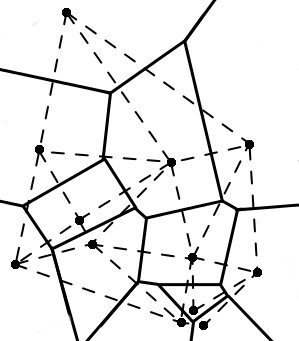
\includegraphics[width=0.5\linewidth]{voronoi}
	\caption{An example Voronoi diagram for objects on a 2-dimensional space.  The black lines correspond to the borders of the Voronoi region, while the dashed lines correspond to the edges of the Delaunay Triangulation.}
	\label{voro-ex}
\end{figure}


With the components of a DHT defined above, we can now show the relationship between DHTs and the primal-dual problems of Delaunay Triangulation and Voronoi Tessellation.
An example Delaunay Triangulation and Voronoi Tessellation is show in Figure \ref{voro-ex}.

%TODO A one-dimensional voronoi fig as example
We can map a given node's ID to a point in a space and the set of short peers to the Delaunay Triangulation.
This would make the range of keys a node is responsible correspond to the node's Voronoi region.
Long peers serve as shortcuts across the mesh formed by Delaunay Triangulation.


Thus, if we can calculate the Delaunay Triangulation between nodes in a DHT, we have a generalized means of creating the overlay network.
This can be done with any algorithm that calculates the Delaunay Triangulation.

Computing the Delaunay Triangulation and/or the Voronoi Tessellation of a set of points is a well analyzed problem.
Many algorithms exist which efficiently compute a Voronoi Tessellation for a given set of points on a plane, such as Fortune's sweep line algorithm \cite{fortune1987sweepline}.

However, DHTs are completed decentralized, with no single node having global knowledge of the topology.
Many of the algorithms to compute Delaunay Triangulation and/or Voronoi Tessellation are unsuited to a distributed environment.
In addition, the computational cost increases when we move into spaces with greater than two dimensions.
In general, finding the Delaunay Triangulation of $n$ points in a space with $d$ dimensions takes $O(n^{\frac{2d-1}{d}})$ time \cite{watson1981computing}.
We use DGVH as the base algorithim for building UrDHT

Candidates are gathered via a gossip protocol as well as notifications from other peers.
How long peers are handled depends on the particular DHT implementation.
This process is described more in Section \ref{sec:protocol}.

The expected maximum size of $ candidates $ corresponds to the expected maximum degree of a vertex in a Delaunay Triangulation.
This is  $\Theta(\frac{\log n}{\log \log n} )$, regardless of the number of the dimensions \cite{bern1991expected}. 
We can therefore expect \textit{short peers} to be bounded by $\Theta(\frac{\log n}{\log \log n})$.

The expected worst case cost of DGVH is \(O(\frac{\log^{4} n}{\log^{4} \log n} )\) \cite{dgvh}, regardless of the dimension \cite{dgvh}.\footnote{As mentioned in the previous footnote, if we are exchanging only short peers with a single neighbor rather than all our neighbors, the cost lowers to \(O(\frac{\log^{2} n}{\log^{2} \log n} )\).}
In most cases, this cost is much lower.
Additional details can be found in our previous work \cite{dgvh}.




We have tested DGVH on Chord (a ring-based topology), Kademlia (an XOR-based tree topology), general Euclidean spaces, and even in a hyperbolic geometry.
This is interesting because not only can we implement the contrived topologies of existing DHTs, but more generalizable topologies like Euclidean or hyperbolic geometries.
We show in Section \ref{sec:experiments} that DGVH works in all of these spaces.
DGVH only needs the distance function to be defined in order for nodes to perform lookup operations and determine responsibility.
%TODO This is where we need to match vocab
%\begin{itemize}
%	\item \textbf{A \texttt{distance} function } - This measures distance in the overlay formed by the Distributed Hash Table.
%	In most DHTs, the distance in the overlay has no correlation with real-world attributes.
%	
%	\item \textbf{A \texttt{responsibility} definition}  This defines the range of keys a node is responsible for. 
%	Not every DHT defines which node is responsible for particular keys in the same way. 
%	For example, nodes in Kademlia are responsible for the keys closest to themselves, while in Chord, nodes are responsible for the keys falling between themselves and the preceding node.
%\end{itemize}
We will now show how we used this information and heuristic to create UrDHT, our abstract model for distributed hash tables.





\section{UrDHT}
\label{sec:urdht}


The name UrDHT comes from the German prefix \textit{ur}, which means ``original.'' 
The name is inspired by UrDHT's ability to reproduce the topology of other distributed hash tables.

UrDHT is divided into 3 broad components: Storage, Networking, and Logic.
Storage handles file storage and Networking dictates the protocol for how nodes communicate.
These components oversee the lower level mechanics of how files are stored on the network and how bits are transmitted through the network.
The specifics are outside the scope of the paper, but can be found on the UrDHT Project site \cite{urdht}.

Most of our discussion will focus on the Logic component.
The Logic component is what dictates the behavior of nodes within the DHT and the construction of the overlay network.
It is composed of two parts: the DHT Protocol and the Space Math.

The DHT Protocol contains the canonical operations that a DHT performs, while the Space Math is what effectively distinguishes one DHT from another.
A developer only needs to change the details of the \texttt{space math} package in UrDHT to create a new type of DHT.
We discuss each in further detail below.

\subsection{The DHT Protocol }
\label{sec:protocol}

The DHT Protocol (\texttt{LogicClass.py}) \cite{urdht} is the shared functionality between every single DHT.
It consists of the node's information, the short peer list that defines the minimal overlay, the long peers that make efficient routing possible, and all the functions that use them.
There is no need for a developer to change anything in the DHT Protocol, but it can be modified if so desired.
The DHT Protocol depends on functions from Space Math in order to perform operations within the specified space.

Many of the function calls should be familiar to anyone who has study DHTs.
We will discuss a few new functions we added and the ones that contribute to node maintenance.



The first thing we note is the absence of \texttt{lookup}.
In our efforts to further abstract DHTs, we have replaced \texttt{lookup} using the function \texttt{seek}.
The \texttt{seek} function acts a single step of \texttt{lookup}.
It returns the closest node to $ key $ that the node knows about.

Nodes can perform \texttt{lookup} by iteratively calling \texttt{seek} until it receives the same answer twice.
We do this because we make no assumptions as to how a client using a DHT would want to perform lookups and handle errors that can occur.
It also means that a single client implementing \texttt{lookup} using iterative \texttt{seek} operations could traverse any DHT topology implemented with UrDHT.

%We also slightly modified the assumptions of how \texttt{join} works.
%The \texttt{join} operation takes in a set of bootstrap nodes, called $ candidates$, rather than a single node.
%%This is part of our plans about how UrDHT can be used as a bootstrap network by providing bootstrapping information for a particular network.
%%We expect nodes that want to join a particular network to be able to query UrDHT and receive a list of nodes that they can use to bootstrap the joining.
%
%The joining node randomly selects one of these $ candidates $ and finds the ``parent'' node currently responsible for the space.
%The joining node then populates its short peers using the ``parent'' node's short peers.
%The node  uses the parent to populate its short peer list and then makes it aware of its existence using \texttt{notify}.
%Once that has been finished, the joining node starts its maintenance thread.
%
%


Maintenance is done via gossip.
Each maintenance cycle, the node recalculates its Delaunay (short) peers using its neighbors' peer lists and any nodes that have notified it since the last maintenance cycle.
Short peer selection are done using DGVH by default.
While DGVH has worked in every single space we have tested, this is not proof it will work in every single case.
It is reasonable and expected that some spaces may require a different Delaunay Triangulation calculation or approximation method.

Once the short peers are calculated, the node handles modifying its long peers.
This is done using the \texttt{handleLongPeers} function described in Section \ref{sec:space}.

\subsection{The Space Math}
\label{sec:space}
The Space Math consists of the functions that define the DHT's topology.
It requires a way to generate short peers to form a routable overlay and a way to choose long peers.
%We use DGVH for generating short peers, which works in every space tested.
Space Math requires the following functions when using DGVH:

\begin{itemize}

%\subsubsection{IDToPoint}
\item The \texttt{idToPoint} function takes in a node's ID and any other attributes needed to map an ID onto a point in the space.
The ID is generally a large integer generated by a cryptographic hash function.
%In the vast majority of DHTs, this \texttt{idToPoint} function needs nothing more than the ID as input.
%The ID is directly translated into a large integer and used as a coordinate in a one dimensional space.


%\subsubsection{Distance}
\item The \texttt{distance} function takes in two points, $a$ and $b$, and outputs the shortest distance from $a$ to $b$.
This distinction matters, since distance is not symmetric in every space.
The prime example of this is Chord, which operates in a unidirectional toroidal ring.



%\subsubsection{Get Closest}
%Depending on what you want to measure, \texttt{getClosest} might measure the distance from $ center$ to each of the candidates or from each of the candidates to the $ center$.

%\subsubsection{Get Delaunay (short) Peers}
\item We use the above functions to implement \texttt{getDelaunayPeers}.
Given a set of points, the $ candidates$, and a center point $ centers$, \texttt{getDelaunayPeers} calculates a mesh that approximates the Delaunay peers of $ center$.
We assume that this is done using DGVH (Algorithm \ref{alg:dgvh}).



\item The function \texttt{getClosest} returns the point closest to $ center$ from a list of $ candidates$, measured by the distance function.
The \texttt{seek} operation depends on the \texttt{getClosest} function.


%\subsubsection{Handle Long Peers}



\item The final function is \texttt{handleLongPeers}.
\texttt{handleLongPeers} takes in a list of $ candidates $ and a $ center$, much like \texttt{getDelaunayPeers}, and returns a set of peers to act as the routing shortcuts.

The implementation of this function should vary greatly from one DHT to another.
For example, Symphony \cite{symphony} and other small-world networks \cite{kleinberg2000navigation} choose long peers using a probability distribution.
Chord has a much more structured distribution, with each long peer being increasing powers of 2 distance away from the node \cite{chord}.
The default behavior is to use all candidates not chosen as short peers as long peers, up to a set maximum.
If the size of long peers would exceed this maximum, we instead choose a random subset of the maximum size, creating a naive approximation of the long links in the Kleinberg small-world model \cite{kleinberg2000navigation}.
Long peers do not greatly contribute to maintenance overhead, so we chose 200 long peers as a default maximum.

%In some case it may more convenient implement \texttt{handleLongPeers} as part of \texttt{getDelaunayPeers}.

\end{itemize}


%\subsubsection*{Put and Poll}
%The functions of \texttt{store} and \texttt{get} can be further abstracted otu to \texttt{put} and \texttt{poll}


%This does X


\section{Implementing other DHTs}
\label{sec:implement}
\subsection{Implementing Chord}

Ring topologies are fairly straightforward since they are one dimensional Voronoi Tessellations, splitting up what is effectively a modular number line among multiple nodes.

Chord uses a unidirectional distance function.
Given two integer keys $ a $ and $ b $ and a maximum value $ 2^{m}$, the \texttt{distance} from $ a $ to $ b $ in Chord is: 
\[ distance(a,b) =
\begin{cases}
	2^m + b - a, & \text{if } b - a < 0 \\
	b-a, & \text{otherwise}
\end{cases}
  \]


Short peer selection is trivial in Chord, so rather than using DGVH for \texttt{getDelaunayPeers}, each node chooses from the list of candidates the candidate closest to it (predecessor) and the candidate to which it is closest (successor).

Chord's finger (long peer) selection strategy is emulated by \texttt{handleLongPeers}.
For each of the $i$th bits in the hash function, we choose a long peer $ p_i $ from the candidates such that 


\[ p_i =   getClosest\left(candidates, t_{i}\right)  \]
where
\[t_{i} =  (n + 2^{i}) \mod 2^m \]
for the current node $n$.
The \texttt{getClosest} function in Chord should return the candidate with the shortest distance from the candidate to the point.

This differs slightly from how selects its long peers.
In Chord, nodes actively seek out the appropriate long peer for each  corresponding bit.
In our emulation, this information is propagated along the ring using short peer gossip.


%for i in range(0, HASHBASE):
%target = tuple([(center[0] + 2**i) % HASHMAX])
%subject = min(others, key=lambda x: chordDist(x.loc, target))
%We know Chord's invariants are not (citation), but our protocol isn't affected by these constraints


\subsection{Implementing Kademlia}
Kademlia uses the exclusive or, or XOR, metric for distance.
This metric, while non-euclidean, is perfectly acceptable for calculating distance.
For two given keys $ a $ and $ b $

\[ distance(a, b) = a  \oplus b\]

The \texttt{getDelaunayPeers} function uses DGVH as normal to choose the short peers for node $n$.
We then used Kademlia's $k$-bucket strategy \cite{kademlia} for \texttt{handleLongPeers}.
The remaining candidates are placed into buckets, each capable holding a maximum of $k$ long peers.

To summarize briefly, node $n$ starts with a single bucket containing itself, covering long peers for the entire range.
When attempting to add a candidate to a bucket already containing $k$ long peers, if the bucket contains node $n$, the bucket is split into two buckets, each covering half of that bucket's range.
Further details of how Kademlia $k$-buckets work can be found in the Kademlia protocol paper \cite{kademlia}.


\subsection{ZHT}
ZHT \cite{li2013zht} leads to an extremely trivial implementation in UrDHT.
Unlike other DHTs, ZHT assumes an extremely low rate of churn.
It bases this rationale on the fact that tracking $ O(n) $ peers in memory is trivial.
This indicates the $ O( \log n)  $  memory  requirement for other DHTs is overzealous and not based on a memory limitation.
Rather, the primary motivation for keeping a number of peers in memory is more due to the cost of maintenance overhead.
ZHT shows, that by assuming low rates of churn (and infrequent maintenance messages as a result), having $O(n)$ peers is a viable tactic for faster lookups.

As a result, the topology of ZHT is a clique, with each node having an edge to all other nodes.
This yields $ O(1) $ lookup times with an $ O(n) $ memory cost.
The only change that needs to be made to UrDHT is to accept all peer candidates as short peers.

\subsection{Implementing a DHT in a non-contrived Metric Space}

We used a Euclidean geometry as the default space when building UrDHT and DGVH \cite{dgvh}.
For two vectors $\vec{a}$ and $\vec{b}$ in $d$ dimensions: 

\[distance\left(\vec{a}, \vec{b}\right) = \sqrt{\sum\limits_{i\in d} \left(a_i-b_i\right)^2}\]


We implement \texttt{getDelaunayPeers} using DGHV and set the minimum number of short peers to $3d+1$, a value we found through experimentation \cite{dgvh}.

Long peers are randomly selected from the left-over candidates after DGVH is performed \cite{dgvh}.
The maximum size of long peers is set to $(3d+1)^2$, but it can be lowered or eliminated if desired and maintain $ O(\sqrt[d]{n}) $ routing time.


Generalized spaces such as Euclidean space allow the assignment of meaning to arbitrary dimension and allow for the potential for efficient querying of a database stored in a DHT.

%\subsection{Implementing a DHT in a Hyperbolic Geometry}
	
\label{sec:hyper}

We have already shown with Kademlia that UrDHT can operate in a non-Euclidean geometry.
Another non-euclidean geometry UrDHT can work in is a hyperbolic geometry.

We implemented a DHT within a hyperbolic geometry using a Poincar\`{e} disc model.
To do this, we implemented \texttt{idToPoint} to create a random point in Euclidean space from a uniform distribution.
This point is then mapped to a Poincar\`{e} disc model to determine the appropriate Delaunay peers.
For any two given points $a$ and $b$ in a Euclidean vector space, the \texttt{distance} in the  Poincar\`{e} disc is:


\[ distance(a, b) = \operatorname{arcosh} \left(  1+ 2 \frac{ \left\| a - b \right\| ^{2} }{ ( 1 - \left\| a \right\| ^{2} ) ( 1 - \left\| b \right\| ^{2} ) }\right) \]


Now that we have a \texttt{distance} function, DGVH can be used in \texttt{getDelaunayPeers} to generate an approximate Delaunay Triangulation for the space.
The \texttt{getDelaunayPeers} and \texttt{handleLongPeers} functions are otherwise implemented exactly as they were for Euclidean spaces. 




Implementing a DHT in hyperbolic geometry has many interesting implications.
Of particular note, embedding into hyperbolic spaces allows us to explore accurate embeddings of internode latency into the metric space \cite{kleinberg2007geographic} \cite{cvetkovski2009hyperbolic}.
This has the potential to allow for minimal latency DHTs.


%\subsection{Services}
%
%There needs to be an easy way to append data to the bootstrapping list.
%
%To do this, we introduce the \texttt{put} and  \texttt{poll} primitives.
%These functions can considered abstracted versions.
%	
\section{Experiments}
\label{sec:experiments}

We use simulations to test our implementations of DHTs using UrDHT.
Using simulations to test the correctness and relative performance of DHTs is standard practice for testing and analyzing DHTs \cite{kademlia} \cite{symphony} \cite{chord}  \cite{tapestry}  \cite{raynet}

%Tests
%k connected randomly populated network
%vars:
%k for your k connected network 10, 20
%duration what we have works
%size 100, 500, 1000, 5000 if possible,
%
%Iterative joins, start with one node
%vars:  join rate (ticks per join) ,1 3 
%final size  100, 500, 1000, 5000 if possible,
%join method (bootstrapping size)  all,
%
%outputs
%Network diameter at tick
%avg greedy routing distance
%greedy routing success rate at tick
%maximum degree
%mean degree
%std deviatation degree
%Anything we want for degree
%
%
%Graph max degree vs expected  maximimum degree  (this is short peers)

%\subsection{Experimental Setup}
We tested four different topologies: Chord, Kademlia, a Euclidean geometry, and a Hyperbolic geometry.
For Kademlia, the size of the $k$-buckets was 3.
In the Euclidean and Hyperbolic geometries, we set a minimum of 7 short peers and a maximum of 49 long peers.

We created 500 node networks, starting with a single node and adding a node each maintenance cycle.\footnote{We varied the amount of maintenance cycles between joins in our experiments, but found it had no effect upon our results.}

For each topology, at each step, we measured:
\begin{itemize}
	\item The average degree of the network.  This is the  number of outgoing links and includes both short and long peers.
	\item The worst case degree of the network.
	\item The average number of hops between nodes using greedy routing.
	\item The diameter of the network.  
	This is the worst case distance between two nodes using greedy routing.
\end{itemize}

We also tested the reachability of nodes in the network.
At every step, the network is fully reachable.

Results generated by the Chord and Kademlia simulations were in line with those from previous work  \cite{kademlia} \cite{chord}.
This demonstrates that UrDHT is capable of accurately emulating these topologies.
We show these results in Figures \ref{fig:ChordDegree} - \ref{fig:KademliaDistance}.



\begin{figure}
	\centering
	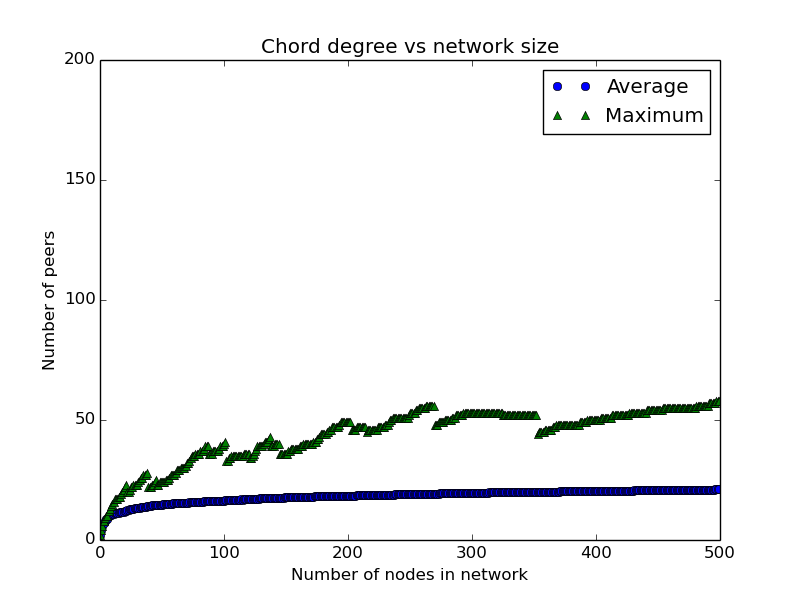
\includegraphics[width=0.75\linewidth]{figs/ChordDegree}
	\caption{This is the average and maximum degree of nodes in the Chord network. This Chord network utilized a 120 bit hash and thus degree is bound at 122 (full fingers, predecessor and successor) when the network reaches $2^{120}$ nodes.}
	\label{fig:ChordDegree}
\end{figure}

\begin{figure}
	\centering
	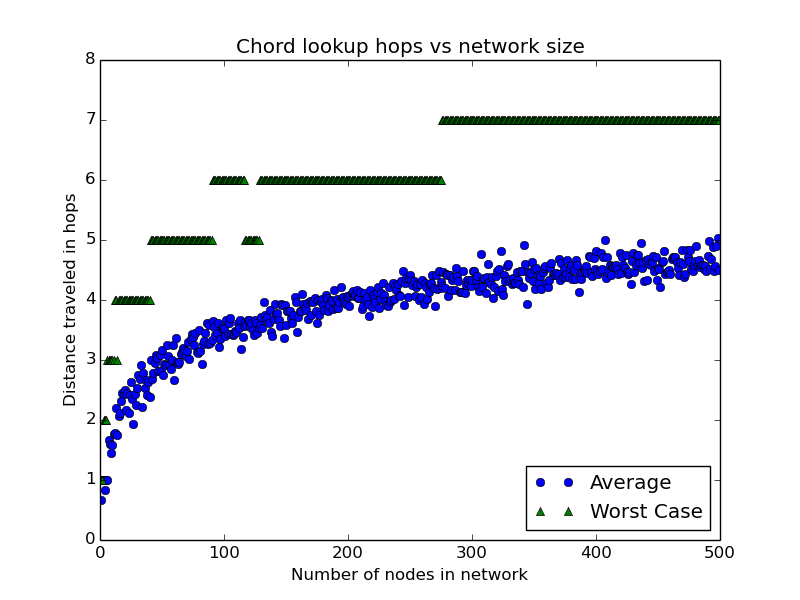
\includegraphics[width=0.75\linewidth]{figs/ChordDistance}
	\caption{This is the number hops required for a greedy routed lookup in Chord. The average lookup between two nodes follows the expected logarithmic curve.}
	\label{fig:ChordDistance}
\end{figure}

\begin{figure}
	\centering
	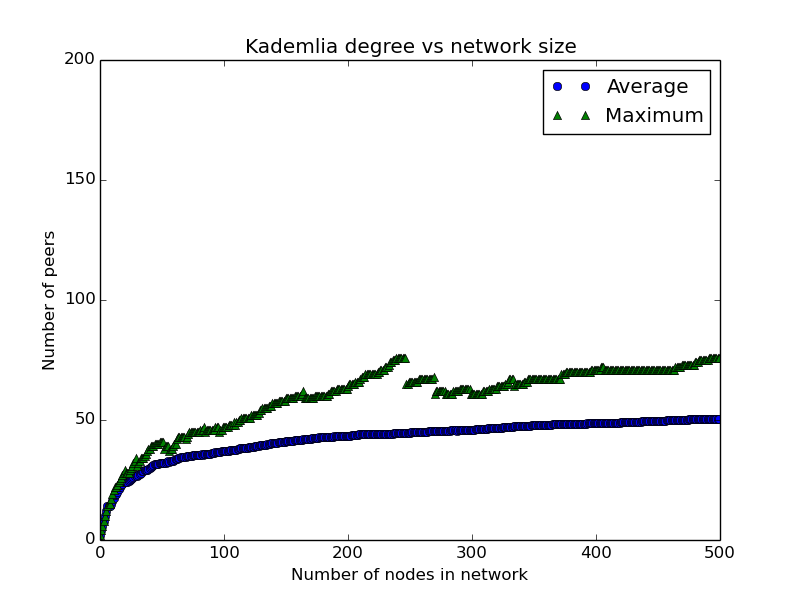
\includegraphics[width=0.75\linewidth]{figs/KademliaDegree}
	\caption{This is the average and maximum degree of nodes in the Kademlia network as new nodes are added.  Both the maximum degree and average degree are $O(\log n)$.}
	\label{fig:KademliaDegree}
\end{figure}
\begin{figure}
	\centering
	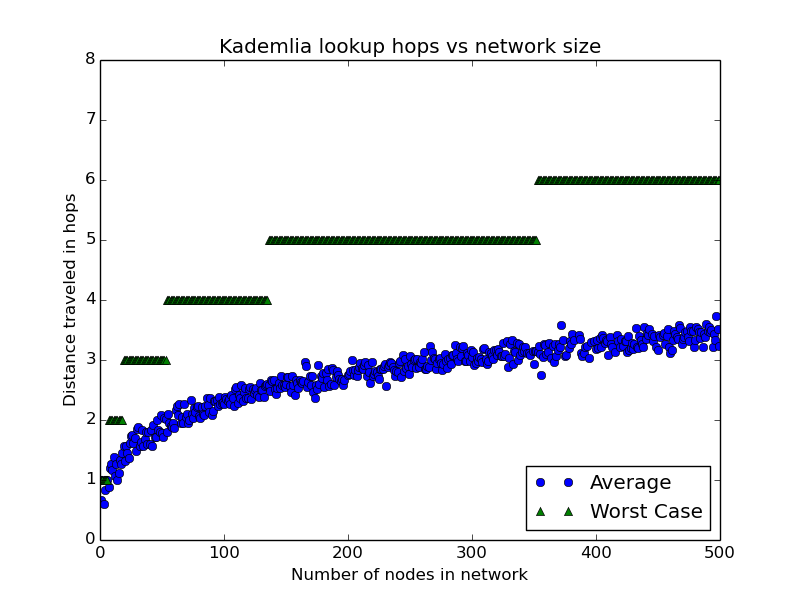
\includegraphics[width=0.75\linewidth]{figs/KademliaDistance}
	\caption{Much like Chord, the average degree follows a distinct logarithmic curve, reaching an average distance of approximately three hops when there are 500 nodes in the network.}
	\label{fig:KademliaDistance}
\end{figure}



The results of our Euclidean and Hyperbolic geometries indicate similar asymptotic behavior: a higher degree produces a lower diameter and average routing. 
However, the ability to leverage this trade-off is limited by the necessity of maintaining an $ O(\log n $) degree.
These results are shown in Figures \ref{fig:EucldianDegree} - \ref{fig:HyperbolicDistance}.

While we maintain the number of links must be $ O(\log n)$, all DHTs practically bound this number by a constant.  
For example, in Chord, this is the number of bits in the hash function plus the number of predecessors/successors.
Chord and Kademlia fill this bound asymptotically. 
The long peer strategy used by the Euclidean and Hyperbolic metrics aggressively filled to this capacity, relying on the distribution of long peers to change as the network increased in size rather than increasing the number of utilized long peers.
This explains why the Euclidean and Hyperbolic spaces have more peers (and thus lower diameter) for a given network size.
This presents a strategy for trade-off of the network diameter vs. the overhead maintenance cost.


%\subsection{Chord}
%Our model of Chord
%\cite{chord}.


\begin{figure}
\centering
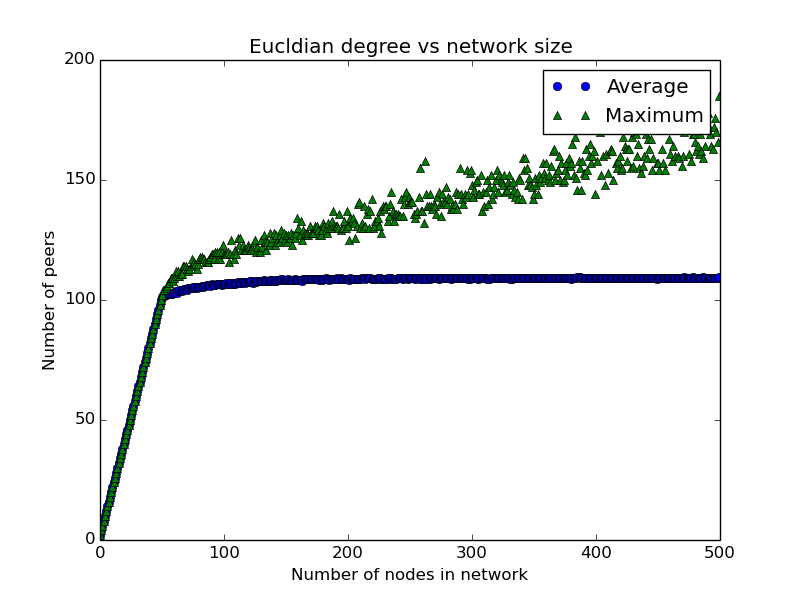
\includegraphics[width=0.75\linewidth]{figs/EucldianDegree}
\caption{Because the long peers increase linearly to the maximum value (49), degree initially rises quickly and then grows  more slowly as the number of long peers ceases to grow and the size short peers increases with network size. }
\label{fig:EucldianDegree}
\end{figure}

\begin{figure}
\centering
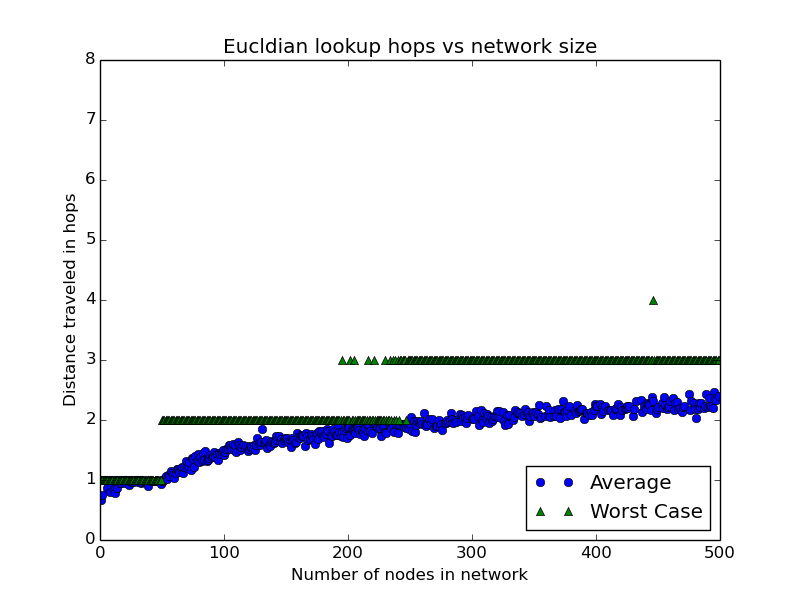
\includegraphics[width=0.75\linewidth]{figs/EucldianDistance}
\caption{The inter-node distance stays constant at 1 until long peers are filled, then rises at the rate of a randomly connected network due to the distribution of long peers selected}
\label{fig:EucldianDistance}
\end{figure}

\begin{figure}
\centering
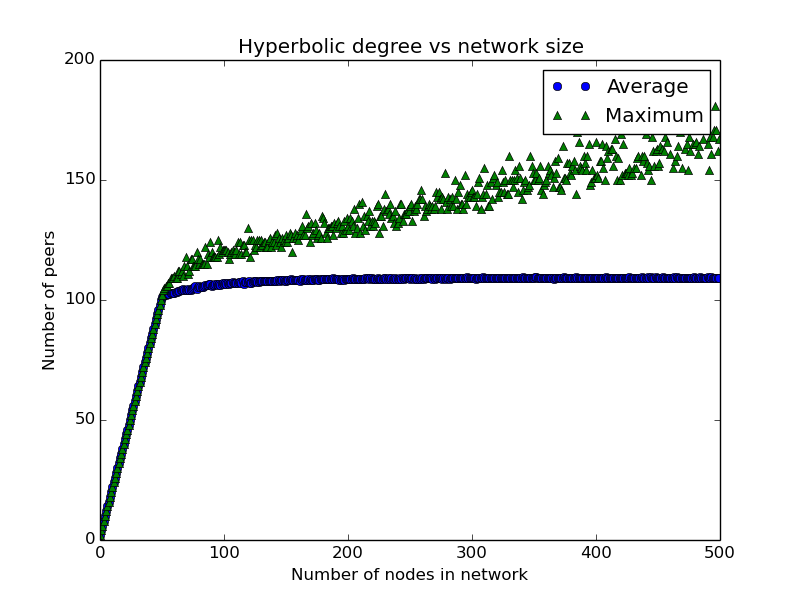
\includegraphics[width=0.75\linewidth]{figs/HyperbolicDegree}
\caption{The Hyperbolic network uses the same long and short peer strategies to the Euclidean network, and thus shows similar results.}
\label{fig:HyperbolicDegree}
\end{figure}
\begin{figure}
\centering
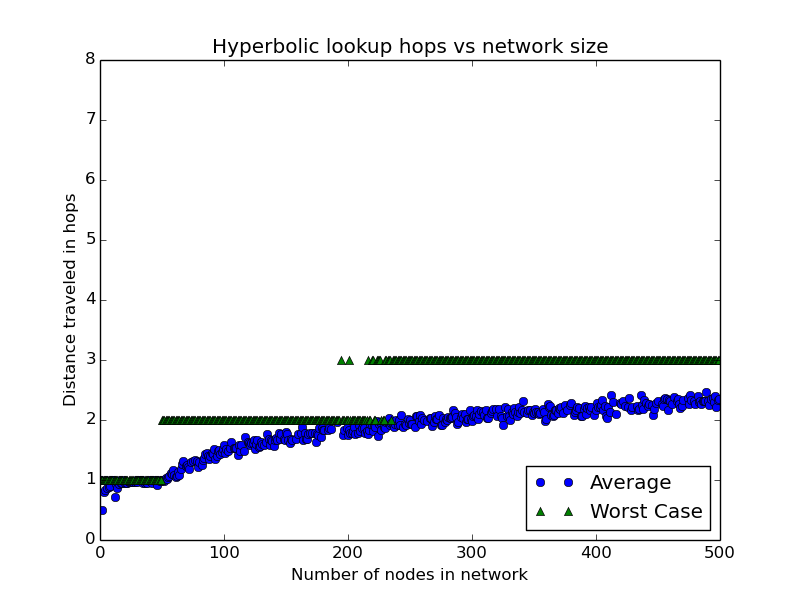
\includegraphics[width=0.75\linewidth]{figs/HyperbolicDistance}
\caption{Like the Euclidean Geometry, our Poincar\`{e} disc based topology has much shorter maximum and average distances.
}
\label{fig:HyperbolicDistance}
\end{figure}


\section{Related Work}\label{sec:related}

There have been a number of efforts to either create abstractions of DHTs or ease the development of DHTs.
One area of previous work focused on constructing overlay networks using system called P2 \cite{loo2005implementing}.
P2 is a network engine for constructing overlays which uses the Overlog declarative logic language.
Writing programs for P2 in Overlog yields extremely concise and modular implementations of for overlay networks. 

Our work differs in that P2 attempts to abstract overlays and ease construction by using a language and framework. while UrDHT focuses on abstracting the idea of a structured overlay into Voronoi Tessellations and Delaunay Triangulations.
This allows developers to define the overlays they are building by mathematically defining a short number of functions.

Our use case is also subtly different. 
P2 focuses on overlays in general, all types of overlays.
UrDHT concerns itself solely with distributed hash tables, specifically, overlays that rely on hash functions to distribute the load of the network and assign responsibility in an autonomous manner. 

One difficulty in using P2 is that it is no longer supported as a project \cite{loo2005implementing}. 
P2's concise Overlog statements also present a sharp learning curve for many developers.
These present challenges not seen with UrDHT.


The T-Man\cite{jelasity2005t} and Vicinity \cite{voulgaris2005epidemic} protocols both present gossip-based methods for organizing overlay networks.
The idea behind T-Man is similar to UrDHT, but again it focuses on overlays in general, while UrDHT applies specifically to DHTs.
% T-man boasts the topology can change at run-time as the needs demand. 
The ranking function is similar to the metrics used by UrDHT using DGVH, but DGVH guarantees full connectivity in all cases and is based on the inherent relationship between Voronoi Tessellations, Delaunay Triangulations, and DHTs.

UrDHT uses a gossiping protocol similar to the ones presented by T-Man and Vicinity due to they gossip protocol's ability to rapidly adjust changes in the topology.


\section{Applications and Future Work}
\label{sec:future}

%Restate the intro
We presented UrDHT, a unified model for DHTs and framework for building distributed applications.
We have shown how it possible to use UrDHT to not only implement traditional DHTs such as Chord and Kademlia, but also in much more generalized spaces such as Euclidean and Hyperbolic geometries.
The viability of UrDHT to utilize Euclidean and Hyperbolic metric spaces indicates that further research into potential topologies of DHTs and potential applications of these topologies is warranted.


%Future improvements of UrDHT would further disconnect long peers and short peers giving them their own implementation cycle.

%Future stuff
There are numerous routes we can take with our model.
Of particular interest are the applications of building a DHT overlay that operates in a hyperbolic geometry.

One of the other features shared by nearly every DHT is that routing works by minimizing the number of hops across the overlay network, with all hops treated as the same length.
This is done because it is assumed that DHTs know nothing about the state of actual infrastructure the overlay is built upon.

However, this means that most DHTs could happily route a message from one continent to another and back.
This is obviously undesirable, but it is the status quo in DHTs.
The reason for this stems from the generation of node IDs in DHTs. 
Nodes are typically assigned a point in the range of a cryptographic hash function. 
The ID corresponds to the hash of some identifier or given a point randomly.
This is done for purposes of load balancing and fault tolerance.

For future work, we want to see if there is a means of embedding latency into the DHT, while still maintaining the system's fault tolerance.
Doing so would mean that the hops traversed to a destination are, in fact, the shortest path to the destination.

We believe we can embed a latency graph in a hyperbolic space and define UrDHT such that it operates within this space \cite{kleinberg2007geographic} \cite{cvetkovski2009hyperbolic}.
The end result would be a DHT with latency embedded into the overlay.
Nodes would respond to changes in latency and the network by rejoining the network at new positions.
This approach would maintain the decentralized strengths of DHTs, while reducing overall delay and communication costs.
%We use  a force spring model to accomplish this.



%Hyperbolic spaces allow us to cleanly embed scale free graphs

%\bibliography{mine,dht,voronoi}
%\bibliographystyle{IEEEtran}

	
%% bare_jrnl.tex
%% V1.4b
%% 2015/08/26
%% by Michael Shell
%% see http://www.michaelshell.org/
%% for current contact information.
%%
%% This is a skeleton file demonstrating the use of IEEEtran.cls
%% (requires IEEEtran.cls version 1.8b or later) with an IEEE
%% journal paper.
%%
%% Support sites:
%% http://www.michaelshell.org/tex/ieeetran/
%% http://www.ctan.org/pkg/ieeetran
%% and
%% http://www.ieee.org/

%%*************************************************************************
%% Legal Notice:
%% This code is offered as-is without any warranty either expressed or
%% implied; without even the implied warranty of MERCHANTABILITY or
%% FITNESS FOR A PARTICULAR PURPOSE!
%% User assumes all risk.
%% In no event shall the IEEE or any contributor to this code be liable for
%% any damages or losses, including, but not limited to, incidental,
%% consequential, or any other damages, resulting from the use or misuse
%% of any information contained here.
%%
%% All comments are the opinions of their respective authors and are not
%% necessarily endorsed by the IEEE.
%%
%% This work is distributed under the LaTeX Project Public License (LPPL)
%% ( http://www.latex-project.org/ ) version 1.3, and may be freely used,
%% distributed and modified. A copy of the LPPL, version 1.3, is included
%% in the base LaTeX documentation of all distributions of LaTeX released
%% 2003/12/01 or later.
%% Retain all contribution notices and credits.
%% ** Modified files should be clearly indicated as such, including  **
%% ** renaming them and changing author support contact information. **
%%*************************************************************************


% *** Authors should verify (and, if needed, correct) their LaTeX system  ***
% *** with the testflow diagnostic prior to trusting their LaTeX platform ***
% *** with production work. The IEEE's font choices and paper sizes can   ***
% *** trigger bugs that do not appear when using other class files.       ***                          ***
% The testflow support page is at:
% http://www.michaelshell.org/tex/testflow/



\documentclass[journal]{IEEEtran}
%
% If IEEEtran.cls has not been installed into the LaTeX system files,
% manually specify the path to it like:
% \documentclass[journal]{../sty/IEEEtran}





% Some very useful LaTeX packages include:
% (uncomment the ones you want to load)


% *** MISC UTILITY PACKAGES ***
%
%\usepackage{ifpdf}
% Heiko Oberdiek's ifpdf.sty is very useful if you need conditional
% compilation based on whether the output is pdf or dvi.
% usage:
% \ifpdf
%   % pdf code
% \else
%   % dvi code
% \fi
% The latest version of ifpdf.sty can be obtained from:
% http://www.ctan.org/pkg/ifpdf
% Also, note that IEEEtran.cls V1.7 and later provides a builtin
% \ifCLASSINFOpdf conditional that works the same way.
% When switching from latex to pdflatex and vice-versa, the compiler may
% have to be run twice to clear warning/error messages.






% *** CITATION PACKAGES ***
%
%\usepackage{cite}
% cite.sty was written by Donald Arseneau
% V1.6 and later of IEEEtran pre-defines the format of the cite.sty package
% \cite{} output to follow that of the IEEE. Loading the cite package will
% result in citation numbers being automatically sorted and properly
% "compressed/ranged". e.g., [1], [9], [2], [7], [5], [6] without using
% cite.sty will become [1], [2], [5]--[7], [9] using cite.sty. cite.sty's
% \cite will automatically add leading space, if needed. Use cite.sty's
% noadjust option (cite.sty V3.8 and later) if you want to turn this off
% such as if a citation ever needs to be enclosed in parenthesis.
% cite.sty is already installed on most LaTeX systems. Be sure and use
% version 5.0 (2009-03-20) and later if using hyperref.sty.
% The latest version can be obtained at:
% http://www.ctan.org/pkg/cite
% The documentation is contained in the cite.sty file itself.






% *** GRAPHICS RELATED PACKAGES ***
%
\ifCLASSINFOpdf
  \usepackage[pdftex]{graphicx}
  % declare the path(s) where your graphic files are
  \graphicspath{{./imgs/}}
  % and their extensions so you won't have to specify these with
  % every instance of \includegraphics
  % \DeclareGraphicsExtensions{.pdf,.jpeg,.png}
\else
  % or other class option (dvipsone, dvipdf, if not using dvips). graphicx
  % will default to the driver specified in the system graphics.cfg if no
  % driver is specified.
  % \usepackage[dvips]{graphicx}
  % declare the path(s) where your graphic files are
  % \graphicspath{{../eps/}}
  % and their extensions so you won't have to specify these with
  % every instance of \includegraphics
  % \DeclareGraphicsExtensions{.eps}
\fi
% graphicx was written by David Carlisle and Sebastian Rahtz. It is
% required if you want graphics, photos, etc. graphicx.sty is already
% installed on most LaTeX systems. The latest version and documentation
% can be obtained at:
% http://www.ctan.org/pkg/graphicx
% Another good source of documentation is "Using Imported Graphics in
% LaTeX2e" by Keith Reckdahl which can be found at:
% http://www.ctan.org/pkg/epslatex
%
% latex, and pdflatex in dvi mode, support graphics in encapsulated
% postscript (.eps) format. pdflatex in pdf mode supports graphics
% in .pdf, .jpeg, .png and .mps (metapost) formats. Users should ensure
% that all non-photo figures use a vector format (.eps, .pdf, .mps) and
% not a bitmapped formats (.jpeg, .png). The IEEE frowns on bitmapped formats
% which can result in "jaggedy"/blurry rendering of lines and letters as
% well as large increases in file sizes.
%
% You can find documentation about the pdfTeX application at:
% http://www.tug.org/applications/pdftex





% *** MATH PACKAGES ***
%
\usepackage{amsmath}
% A popular package from the American Mathematical Society that provides
% many useful and powerful commands for dealing with mathematics.
%
% Note that the amsmath package sets \interdisplaylinepenalty to 10000
% thus preventing page breaks from occurring within multiline equations. Use:
%\interdisplaylinepenalty=2500
% after loading amsmath to restore such page breaks as IEEEtran.cls normally
% does. amsmath.sty is already installed on most LaTeX systems. The latest
% version and documentation can be obtained at:
% http://www.ctan.org/pkg/amsmath





% *** SPECIALIZED LIST PACKAGES ***
%
%\usepackage{algorithmic}
% algorithmic.sty was written by Peter Williams and Rogerio Brito.
% This package provides an algorithmic environment fo describing algorithms.
% You can use the algorithmic environment in-text or within a figure
% environment to provide for a floating algorithm. Do NOT use the algorithm
% floating environment provided by algorithm.sty (by the same authors) or
% algorithm2e.sty (by Christophe Fiorio) as the IEEE does not use dedicated
% algorithm float types and packages that provide these will not provide
% correct IEEE style captions. The latest version and documentation of
% algorithmic.sty can be obtained at:
% http://www.ctan.org/pkg/algorithms
% Also of interest may be the (relatively newer and more customizable)
% algorithmicx.sty package by Szasz Janos:
% http://www.ctan.org/pkg/algorithmicx




% *** ALIGNMENT PACKAGES ***
%
%\usepackage{array}
% Frank Mittelbach's and David Carlisle's array.sty patches and improves
% the standard LaTeX2e array and tabular environments to provide better
% appearance and additional user controls. As the default LaTeX2e table
% generation code is lacking to the point of almost being broken with
% respect to the quality of the end results, all users are strongly
% advised to use an enhanced (at the very least that provided by array.sty)
% set of table tools. array.sty is already installed on most systems. The
% latest version and documentation can be obtained at:
% http://www.ctan.org/pkg/array


% IEEEtran contains the IEEEeqnarray family of commands that can be used to
% generate multiline equations as well as matrices, tables, etc., of high
% quality.




% *** SUBFIGURE PACKAGES ***
%\ifCLASSOPTIONcompsoc
%  \usepackage[caption=false,font=normalsize,labelfont=sf,textfont=sf]{subfig}
%\else
%  \usepackage[caption=false,font=footnotesize]{subfig}
%\fi
% subfig.sty, written by Steven Douglas Cochran, is the modern replacement
% for subfigure.sty, the latter of which is no longer maintained and is
% incompatible with some LaTeX packages including fixltx2e. However,
% subfig.sty requires and automatically loads Axel Sommerfeldt's caption.sty
% which will override IEEEtran.cls' handling of captions and this will result
% in non-IEEE style figure/table captions. To prevent this problem, be sure
% and invoke subfig.sty's "caption=false" package option (available since
% subfig.sty version 1.3, 2005/06/28) as this is will preserve IEEEtran.cls
% handling of captions.
% Note that the Computer Society format requires a larger sans serif font
% than the serif footnote size font used in traditional IEEE formatting
% and thus the need to invoke different subfig.sty package options depending
% on whether compsoc mode has been enabled.
%
% The latest version and documentation of subfig.sty can be obtained at:
% http://www.ctan.org/pkg/subfig




% *** FLOAT PACKAGES ***
%
%\usepackage{fixltx2e}
% fixltx2e, the successor to the earlier fix2col.sty, was written by
% Frank Mittelbach and David Carlisle. This package corrects a few problems
% in the LaTeX2e kernel, the most notable of which is that in current
% LaTeX2e releases, the ordering of single and double column floats is not
% guaranteed to be preserved. Thus, an unpatched LaTeX2e can allow a
% single column figure to be placed prior to an earlier double column
% figure.
% Be aware that LaTeX2e kernels dated 2015 and later have fixltx2e.sty's
% corrections already built into the system in which case a warning will
% be issued if an attempt is made to load fixltx2e.sty as it is no longer
% needed.
% The latest version and documentation can be found at:
% http://www.ctan.org/pkg/fixltx2e


%\usepackage{stfloats}
% stfloats.sty was written by Sigitas Tolusis. This package gives LaTeX2e
% the ability to do double column floats at the bottom of the page as well
% as the top. (e.g., "\begin{figure*}[!b]" is not normally possible in
% LaTeX2e). It also provides a command:
%\fnbelowfloat
% to enable the placement of footnotes below bottom floats (the standard
% LaTeX2e kernel puts them above bottom floats). This is an invasive package
% which rewrites many portions of the LaTeX2e float routines. It may not work
% with other packages that modify the LaTeX2e float routines. The latest
% version and documentation can be obtained at:
% http://www.ctan.org/pkg/stfloats
% Do not use the stfloats baselinefloat ability as the IEEE does not allow
% \baselineskip to stretch. Authors submitting work to the IEEE should note
% that the IEEE rarely uses double column equations and that authors should try
% to avoid such use. Do not be tempted to use the cuted.sty or midfloat.sty
% packages (also by Sigitas Tolusis) as the IEEE does not format its papers in
% such ways.
% Do not attempt to use stfloats with fixltx2e as they are incompatible.
% Instead, use Morten Hogholm'a dblfloatfix which combines the features
% of both fixltx2e and stfloats:
%
% \usepackage{dblfloatfix}
% The latest version can be found at:
% http://www.ctan.org/pkg/dblfloatfix




%\ifCLASSOPTIONcaptionsoff
%  \usepackage[nomarkers]{endfloat}
% \let\MYoriglatexcaption\caption
% \renewcommand{\caption}[2][\relax]{\MYoriglatexcaption[#2]{#2}}
%\fi
% endfloat.sty was written by James Darrell McCauley, Jeff Goldberg and
% Axel Sommerfeldt. This package may be useful when used in conjunction with
% IEEEtran.cls'  captionsoff option. Some IEEE journals/societies require that
% submissions have lists of figures/tables at the end of the paper and that
% figures/tables without any captions are placed on a page by themselves at
% the end of the document. If needed, the draftcls IEEEtran class option or
% \CLASSINPUTbaselinestretch interface can be used to increase the line
% spacing as well. Be sure and use the nomarkers option of endfloat to
% prevent endfloat from "marking" where the figures would have been placed
% in the text. The two hack lines of code above are a slight modification of
% that suggested by in the endfloat docs (section 8.4.1) to ensure that
% the full captions always appear in the list of figures/tables - even if
% the user used the short optional argument of \caption[]{}.
% IEEE papers do not typically make use of \caption[]'s optional argument,
% so this should not be an issue. A similar trick can be used to disable
% captions of packages such as subfig.sty that lack options to turn off
% the subcaptions:
% For subfig.sty:
% \let\MYorigsubfloat\subfloat
% \renewcommand{\subfloat}[2][\relax]{\MYorigsubfloat[]{#2}}
% However, the above trick will not work if both optional arguments of
% the \subfloat command are used. Furthermore, there needs to be a
% description of each subfigure *somewhere* and endfloat does not add
% subfigure captions to its list of figures. Thus, the best approach is to
% avoid the use of subfigure captions (many IEEE journals avoid them anyway)
% and instead reference/explain all the subfigures within the main caption.
% The latest version of endfloat.sty and its documentation can obtained at:
% http://www.ctan.org/pkg/endfloat
%
% The IEEEtran \ifCLASSOPTIONcaptionsoff conditional can also be used
% later in the document, say, to conditionally put the References on a
% page by themselves.




% *** PDF, URL AND HYPERLINK PACKAGES ***
%
%\usepackage{url}
% url.sty was written by Donald Arseneau. It provides better support for
% handling and breaking URLs. url.sty is already installed on most LaTeX
% systems. The latest version and documentation can be obtained at:
% http://www.ctan.org/pkg/url
% Basically, \url{my_url_here}.




% *** Do not adjust lengths that control margins, column widths, etc. ***
% *** Do not use packages that alter fonts (such as pslatex).         ***
% There should be no need to do such things with IEEEtran.cls V1.6 and later.
% (Unless specifically asked to do so by the journal or conference you plan
% to submit to, of course. )


% correct bad hyphenation here
%\hyphenation{op-tical net-works semi-conduc-tor}


\begin{document}
%
% paper title

\title{Replication Strategies to Increase Storage Robustness in Decentralized P2P Architectures}
%
%
% author names and IEEE memberships
% note positions of commas and nonbreaking spaces ( ~ ) LaTeX will not break
% a structure at a ~ so this keeps an author's name from being broken across
% two lines.
% use \thanks{} to gain access to the first footnote area
% a separate \thanks must be used for each paragraph as LaTeX2e's \thanks
% was not built to handle multiple paragraphs
%

\author{Brendan~Benshoof}% <-this % stops a space
\thanks{GSU CS. MBD.}% <-this % stops a space

% note the % following the last \IEEEmembership and also \thanks -
% these prevent an unwanted space from occurring between the last author name
% and the end of the author line. i.e., if you had this:
%
% \author{....lastname \thanks{...} \thanks{...} }
%                     ^------------^------------^----Do not want these spaces!
%
% a space would be appended to the last name and could cause every name on that
% line to be shifted left slightly. This is one of those "LaTeX things". For
% instance, "\textbf{A} \textbf{B}" will typeset as "A B" not "AB". To get
% "AB" then you have to do: "\textbf{A}\textbf{B}"
% \thanks is no different in this regard, so shield the last } of each \thanks
% that ends a line with a % and do not let a space in before the next \thanks.
% Spaces after \IEEEmembership other than the last one are OK (and needed) as
% you are supposed to have spaces between the names. For what it is worth,
% this is a minor point as most people would not even notice if the said evil
% space somehow managed to creep in.



% The paper headers
% The only time the second header will appear is for the odd numbered pages
% after the title page when using the twoside option.
%
% *** Note that you probably will NOT want to include the author's ***
% *** name in the headers of peer review papers.                   ***
% You can use \ifCLASSOPTIONpeerreview for conditional compilation here if
% you desire.




% If you want to put a publisher's ID mark on the page you can do it like
% this:
%\IEEEpubid{0000--0000/00\$00.00~\copyright~2015 IEEE}
% Remember, if you use this you must call \IEEEpubidadjcol in the second
% column for its text to clear the IEEEpubid mark.



% use for special paper notices
%\IEEEspecialpapernotice{(Invited Paper)}




% make the title area
\maketitle

% As a general rule, do not put math, special symbols or citations
% in the abstract or keywords.
\begin{abstract}
The abstract goes here.
\end{abstract}

% Note that keywords are not normally used for peerreview papers.
\begin{IEEEkeywords}

\end{IEEEkeywords}






% For peer review papers, you can put extra information on the cover
% page as needed:
% \ifCLASSOPTIONpeerreview
% \begin{center} \bfseries EDICS Category: 3-BBND \end{center}
% \fi
%
% For peerreview papers, this IEEEtran command inserts a page break and
% creates the second title. It will be ignored for other modes.
\IEEEpeerreviewmaketitle



\section{Introduction}

In this paper, we will consider a selection of strategies to increase robustness of storage in a p2p network.
Each strategy will be described, analyzed and finally compared and contrasted with other strategies.

\section{Robustness}

\subsection{Robustness and Churn}
\subsection{Robustness and network partitions}

\section{Randomized Replication Strategies}

\subsection{k-Replica}
\subsection{Adaptive Replica (IRM)}

\section{Active Replication Strategies}

\subsection{Active Sponsorship}

\subsection{Redundant Subnetworks}

\section{Conclusions}


\end{document}

	

\chapter{Online Hyperbolic Latency Graph Embedding as Synthetic Coordinates for Latency Reduction in Distributed Hash Tables}
%
%
% author names and IEEE memberships
% note positions of commas and nonbreaking spaces ( ~ ) LaTeX will not break
% a structure at a ~ so this keeps an author's name from being broken across
% two lines.
% use \thanks{} to gain access to the first footnote area
% a separate \thanks must be used for each paragraph as LaTeX2e's \thanks
% was not built to handle multiple paragraphs
%
\begin{center}
Brendan~Benshoof, Andrew~Rosen, Dr.~Robert~Harrison
\end{center}



\section{Introduction}

There is an inherent trade-off between availability and latency minimization in DHT design. 
A design that always ensures minimal latency routes is a clique\cite{li2013zht} which requires 1 hop for lookups.

However this design requires all members of the network to maintain $O(n)$ connections, which limits the scalability of such a system.

Distributed Hash Tables seek to ensure the scalability of the system by requiring nodes to track only $O(\log{n})$ nodes in the network, which necessitates higher latency in queries over the Distributed Hash Table.
We present a technique to minimize the maintenance overhead and query latencies within the constraint of maintaining the scalability of the network.

Distributed Hash Tables form the core of many P2P systems like Bitorrent\cite{jimenez2011kademlia}, CJDNS\cite{hodson2013meshnet}, and I2P\cite{zantout2011i2p}.
Increasing the response time and efficiency of DHTs will provide these systems and systems like them with increased performance and capacity to scale to more users.

\section{Background}

The ideas applied in this paper pull from a variety of backgrounds, including wireless networking, graph embedding and hyperbolic geometry.

\subsection{Geographic Routing}

Geographic routing is used in CDN latency optimization and Wireless Sensor Networks\cite{karp2000geographic}.
The basic premise, is unlike traditional network routing mechanism, messages can be routed in a network based on the location of the current node and the location of the destination.
While the ideal is that messages could be routed greedily, the realities of radio and connectivity limitations have resulted in a number of proposed algorithms.

There are serious concerns with application of simple geographic routing in practice.
Geographic locations may not accurately represent network connectivity and latency.
Often holes" or "lakes" in the network prevent greedy routing, requiring more complex and stateful routing methods to act as auxiliary to greedy routing.
The fundamental problem being that due to the inability to make connection past an obstacle 

While we will take inspiration from the mechanisms of greedy geographic routing, distributed hash tables are not vulnerable to the problem of untraversable terrain that plagues wireless sensor networks. 
So while in practice, so long as a greedily traversable graph is maintained, we can use only the greedy geographic forwarding strategy to route messages.
This leaves us with the problem that locations and routes in space often do not match the throughput and latency reality of the network.
The focus of this work is building a coordinate system alternative to geographic location that provides the capacity to leverage greedy geographic routing for both successful and efficient routes.

\subsection{Greedily Traversable Mesh}

The idea of a greedy traversable Mesh is that based on a distance estimator, a route can be found between between any two nodes by greedy best first search without any backtracking.

This provides efficient routing through the network without maintaining any state in the packet or maintaining routing tables.

\subsubsection{DGVH}

DGVH\cite{dgvh} is a technique for building minimal greedy traversable meshes in arbitrary metric spaces (it requires that distances follow the triangle inequality and are symmetric between 2 points)

algorithm for peer selection:
\begin{enumerate}
	\item Given a $center$ node we are finding the Peer List for
	\item Initialize a empty $Peers$ list
	\item Consider the list $Candidates$ of candidate peers sorted by increasing distance from $center$
	\item Pop the closest member of $Candidates$ and add it to the $Peers$ list. $center$ will always peer with the closest node to it.
	\item For the remaining nodes $c$ in $Candiates$
	\begin{enumerate}
		\item if $c$ is closer to $center$ than any current members of $Peers$ then add it to the $Peers$ list
		\item else discard $c$
	\end{enumerate}
\end{enumerate}





\subsection{Scale Free Networks}

Scale free networks are a family of tree-like networks defined by an having expoential  degree distribution, and a tendency for high-degree nodes to be linked to other high degree nodes.

These properties describe a network with a $O(\log{n})$ diameter, which in practical systems can often be considered constant.

Scale free Networks are of interest to us because they are a generalization of the connectivity topology of human build digital networks.
The latency distribution of a representative sample of computer in the global internet should show a latency similar to that of a representative subset of a scale free graph.


\section{Previous Works}

\subsection{Kleinberg's Hyperbolic Embedding}
A distributed and dynamic hyperbolic embedding of latency suitable for optimizing a distributed hash table was envisioned by Robert Kleinberg in 2007.

\subsubsection{Greedy Embedding}
The Greedy Embedding discussed by Kleinberg is inverse to the "DGVH" method of generating a greedy traversable mesh discussed above.
Rather than being given a set of points and generating a traversal mesh, we are given a graph and solve for points for each node such that resulting mesh is greedy traversable.

Initially discussed Papadimitriou et al\cite{papadimitriou2004conjecture} by A greedy embedding can be formally defined as a distance function between two points $d(a,b)$ in a given metric space and a transformation $f(v)$ that maps each vertex in the given graph such that for every pair of non-adjacent vertices $a,v\in G$ there exists a third vertex $c$ adjacent to a such that $d(u,b) < d(a,b)$. 
Essentially, the result of this definition is that for any vertices not directly connected, there exists a path of nodes that iterativly closer to the target that could be followed by greedy traversal (interestingly, graphs produced by DGVH are forced by the algorithm to fulfill this property making it an inverse function to greedy embedding)

\subsubsection{Life on the Hyperbolic Plane}
Hyperbolic space in 2 dimensions is defined as the surface of a hyperbola in 3 dimensions where all paths between points are taken along the surface of the hyperbola.
This hyperbola is defined by the equation $z^{2}=x^{2}+y^{2}+1$.
Note that for any $(x,y)$ pair there exists 2 solutions for the value of $z$, one positive and the other negative.
These two solutions form 2 disconnected "sheets" mirrored across the xy-plane.
By convention we only consider points on the negative z sheet (all calculations and processes work effectively on either sheet as long as all considered points are on the same sheet).

The hyperbolic plane has many differing qualities from the euclidean plane, most importantly is that of "relativity".
On a euclidean plane, we can treat any point as the "origin" and calculate new locations for every point or figure on that plane by translation, and have all inter-point angles and distances remain the same.
The euclidean distance equation $\sqrt{(x_{1}-x_{0})^{2})+(y_{1}-y_{0})^{2})}$ can be interpreted as translating $(x_{1},y_{1})$ into the reference frame where $(x_{1},y_{1})$ is the center, and using the distance metric $\sqrt{x^{2}+y^{2}}$ to determine the distance.
Unlike this, the hyperbolic plane has a defined center, and while points can be rotated and mirrored freely over this center without changing inter-point distance and angle, they cannot be translated.
The distance between two points in the hyperboloid model is $\operatorname{arcosh}(z_{0}z_{1} - x_{0}x_{1} - y_{0}y_{1})$ where $\operatorname{arcosh}x$ is defined as $\ln{(x+\sqrt{x^{2}+1})}$

Unlike euclidean space, a 2d Hyperbolic Plane has a Greedy Embedding for any graph.
Kleinberg presents his technique for building arbitrary graph embedding in hyperbolic spaces by building a spanning tree of the graph, then embedding the tree into the hyperbolic space.
This is effective because the circumference of the disk increases exponentially with radius, therefore we can trivially embed trees into the space as the available space on the disk increases in correspondence with the number of leaves in a full tree.
While greedily traversable, the resulting embedding does not provide desirable qualities in that greedy routes are not necessarily the shortest and central nodes receive high levels on congestion.



\subsection{Greedy Hyperbolic Embedding}
Further work by Papadopoulos et al\cite{papadopoulos2010greedy} shows an greedy centralized technique for managing the creation of a dynamic network in a hyperbolic space.
Papadopoulos presents improvements over Kleinberg's initial work by presenting a simple stratagy for handling node joining the network (greedy insertion) to minimize path latency and routing methods to handle node and edge failure.



\subsubsection{Growing Network with Greedy Embedding}

Papadopoulos et al provide a sophisticated method for accurate generating a growing scale free network in a hyperbolic space. It is important to note that they are creating a new topology and network from scratch, rather than attempting to use existing latency information to build a Greedy Embedding that also represent that network topology.

Papadopoulos et al show that graphs with similar properties to those found in the "nature" of real world network topologies can be generated and have desirable greedy routing properties.
This is accomplished by randomly selecting points in the hyperbolic space such that, all points are constrained within a given disk that represents the network radius and a distribution of radius that represents the branching factor of the scale free graph intended to be simulated.

Points are then connected together randomly, using a model weighted by inter-node distance and angle.

\subsubsection{Utility in building a Hyperbolic DHT}

While interesting, the statistical method of peer selection proposed is insufficent for ensuring a Greedy Embedding that can be navigated under churn. The proposed Gravity-Pressure routing method requires packets maintain an nonviable amount of state information without reasonable benefit.
It begins to follow the path of geographic routing techniques with growing sophistication in response to an environment that is not greedy routable.
We are better served by ensuring the environment it greedy routable than attempting to add overhead to routing to manage failures of topology maintenance.




\section{Contribution}


We present a technique for building a Distributed Hash Table on a hyperbolic metric space to minimize  look-up and maintenance latency within the constrains of ensuring the scalability of the system.
We show a simple greedy method for inserting nodes into the network such that latency is congruent 
with the distance metric.
We show that unlike previous works indicate, no special updating of node location is required in response to the joining or exiting of new nodes and in fact a constant churn rate will help the system respond to changes in global latency distribution.
We have found that if we augment the network topology with a greedy navigable mesh, holes introduced via node loss are accurately repaired and new nodes are greedily inserted at latency ideal locations in the network.

\subsection{The Value of Approximation}
Unlike previous work, in presenting a practical DHT description, we are dealign with different premises than previous work with hyperbolic embedding.
The largest divergence from Kleinberg and Papadopoulos works is that rather than dealing with embedding a scale free graph, we are embedding a effectivly random sampling of a massive scale free graph in the form of the internet.
Secondly, we will be dealing with constant churn of members of the network, and changes in inter-node latnecy over time.
The consequence of this is that the exact methods proposed in previous work, which promise essentially optimial routes cannot be extended into reality in that fashion.
Because we are dealing with a sampling of a scale free graph, rather than the entire graph, we will induce stetch simply because we cannot connect all nodes in the overlay network as a clique. 
We are bound to the scalaibility limitations of a distributed hash table.


\subsection{Hyperbolic DHT Model}

We establish an Hyperbolic DHT Network in the hyperbolic plane using the hyperboloid model. While any hyperbolic plane representation will work effectively, for accurate internal representation we utilize the x,y,z coordinates of points in the 3d hyperbolic sheet rather than poincare disk or similar representations due to the inability of floating point numbers to accurately represent values at the extremes of those models.

%describe the hyperboloid model in detail?

Using a direct application of DGVH's capacity to build greedy traversable overlay networks in arbitrary metric spaces, we can extend the contrived metric spaces of Chord and Kademlia into a more general model. This would allow DHTs to be constructed in any metric with the triangle inequality and symmetric distance. Conveniently, as it is the focus of this paper, the hyperbolic plane metric space is easy for DGVH to utilize.

We will use points on the hyperbolic plane in the hyperboloid representation\cite{jansen1909abbildung} (3d coordinates of points on the bottom sheet of the hyperbola) with the distance metric $\operatorname{arcosh} (z_{0} \cdot z_{1} - x_{0} \cdot x_{1} - y_{0} \cdot y_{1})$

\subsubsection{Joining and Embedding}

The only divergence from a traditional DHT's operation is in the assignment of points in the coordinate space to joining nodes.
To preserve the accuracy of the embedding, we must place nodes in the network at a point where they have low local latency.
Given that the goal of the embedding is that paths can be routed with minimal latency, the leverage the inverse to greedily place nodes into the network.

Given any arbitrary node in the network as a start point, the joining has two sequential greedy searches:

First the joining node greedily searches for the location <0,0,-1> which represents the "center" of the network.
Once we have a reference to a node at the center of the network the preform a greedy best first search similar to before, but rather than looking up the next hop, we query a node for its peers. We then ping each peer to test latency. We select the peer with lowest latency and iterate this process until we have found a node to which we have lower latency than all of its peers. We select a location subordinate to this node and preform a traditional UrDHT join at this location.


\begin{enumerate}
	\item build a greedy navigable mesh over points in the hyperbolic embedding to augment routing and ensure delivery using greedy forwarding under churn
	\item describe a greedy algorithm for joining nodes to discover ideal insertion points starting from any node in the network
\end{enumerate}

\subsection{Routing and Message Passing in the Hyperbolic DHT}
Routing uses a modified "recursive" method.

It is important to note that usage of the overlay network does not provide any increase in efficiency, rather it provides an efficient mechanism for finding the owner of a given location with minimal overhead while preserving the capacity of the network to scale to arbitrary size efficiently. 

A message has a destination location in the hyperbolic space, query message and callback IP and port to return the response to.
Generally a message will be targeted to a specific location in the metric space, rather than a specific server, and whichever server is responsible for that location will handle the query.
Often a message will originate from a user who is not even a member of the DHT querying to store a value or retrieve a stored value.

A message will begin in the network at a selected "sponsor", who hopefully is chosen for low latency with the user, but this is not required and a sponsor can simply be any known member of the DHT.
The message is passed between members of the DHT using a greedy "best first" strategy, that forwards the message to the peer closest to the destination location (in this case using the distance along the geodesic).
No trace-back or hop count information is required to ensure delivery, and a node will consider itself the destination of the message when it is closer to the destination location than any of its peers.
Once the query message is handled (often storing or retrieving a value), the response (a success notification or the requested data) will be sent directly to the user rather than using the overlay network.


\subsection{Storing Records on the Hyperbolic Surface}

The traditional mechanism of mapping keys to cryptographic hashes is less intuitive when locations in the space are actual points rather than integers.
The most straightforward method is to design a pseudo-random point generator, that can be seeded using the more traditional cryptographic hash.
Care must be taken to ensure that the results of this process are evenly distributed.
Using a classical pseudo-random number generator like mersenne-twister with classical 32-bit or 64-bit data types will bound the maximum number of unique locations to the number of unique integers the PRNG can generate, and as the distributed system grows in size increases to the size and format of these identifiers may be required.

As we are using the Hyperboloid model of representing points in hyperbolic plane, we must map our hash values onto the hyperbolic plane with the goals of distributing those point evenly in portions of the plane actually occupied by nodes in the system.
Given a centered and bounded disk on the hyperbolic plane in which all nodes fall, we can expect the distribution of nodes to be linear over the polar angle an exponentially distributed over the radius. 


Using the following algorithm to produce points will evenly distribute the random points over the disk up to MAXRADIUS. A maximum radius is required because a higher share of points will be distributed to locations distant from the origin of the space as the circumference of the space increases exponentially in response to radius. While it would be possible to distribute points over an unbounded space statistically, in this case the majority of points would be assigned to portions of the hyperbolic disk increasingly distant from the embedding of the DHT nodes.  
\begin{enumerate}
	\item SEED(HASH(key))
	\item ANGLE = $2\pi{} \dot{} \mathit{RANDOM()}$
	\item RADIUS = $\mathit{MAXRADIUS} + \frac{\log{(1-{\mathit{RANDOM()}})}}{\mathit{MAXRADIUS}}$
\end{enumerate}


While it is perfectly possible that the network would either be smaller or larger in radius than a pre-chosen MAXRADIUS, the disparity in load due to this is likely a preferable problem then attempting to vary MAXRADIUS at runtime. (If there is an expectation of the network's size at the time of establishment, an appropriate MAXRADIUS can be chosen in respect to that.

No matter what MAXRADIUS is chosen, all keys will be assigned to responsible nodes, however if MAXRADIUS is smaller than the network radius then it is likely nodes on the periphery will not be assigned records (this may be ideal behavior in more general systems than a DHT, as these nodes will likely have high latency)

\section{Analysis}

\subsection{Network Diameter}

We present two independent arguments that the diameter of a greedy traversable graph embedding of a scale-free graph in the hyperbolic plane is $O(\log{n})$

Given that the diameter of a scale free graph is $O(\frac{\log{n}}{\log{\log{n}}})$\cite{bollobas2004diameter} and the greedy embedding is a super-set of this graph (and being a super-set could only reduce the diameter) the diameter of the embedding is $O(\frac{\log{n}}{\log{\log{n}}})$ or better which falls in $O(\log{n})$

Given that the greedy insertion algorithm attempts to uniformly insert nodes into a bounded hyperbolic plane such that the Voronoi regions of these nodes are approximately equal in area.
Area of the hyperbolic disk is effectively a exponential function of the radius, thus the average shortest path in the network is expected to cross $O(\log{n})$ regions.

\subsection{Expected Path Stretch}

The ideal stretch ratio ($\frac{\mathit{Actual Path Length}}{\mathit{Optimal Path Length}}$) for the hyperbolic embedding is $O(1))$.
This stretch is caused by errors in the embedding taking non-optimal routes.
Previous works show that greedy routing in the hyperbolic overlay are $O(1)$
Even if the accuracy of the hyperbolic embedding fails due to unforeseen technical problems or active attack, the properties of the hyperbolic space ensure that the stretch factor is no worse than if nodes were connected randomly as in a traditional DHT.

The stretch ratio observed in existing DHTs is the number of hops required to complete a lookup.
In practice, the distance between any successive hops in the lookup is expected to be the average inter-node distance, thus the expected stretch is $O(\log{n})$ times the average inter-node distance. 

\begin{figure}[H]
	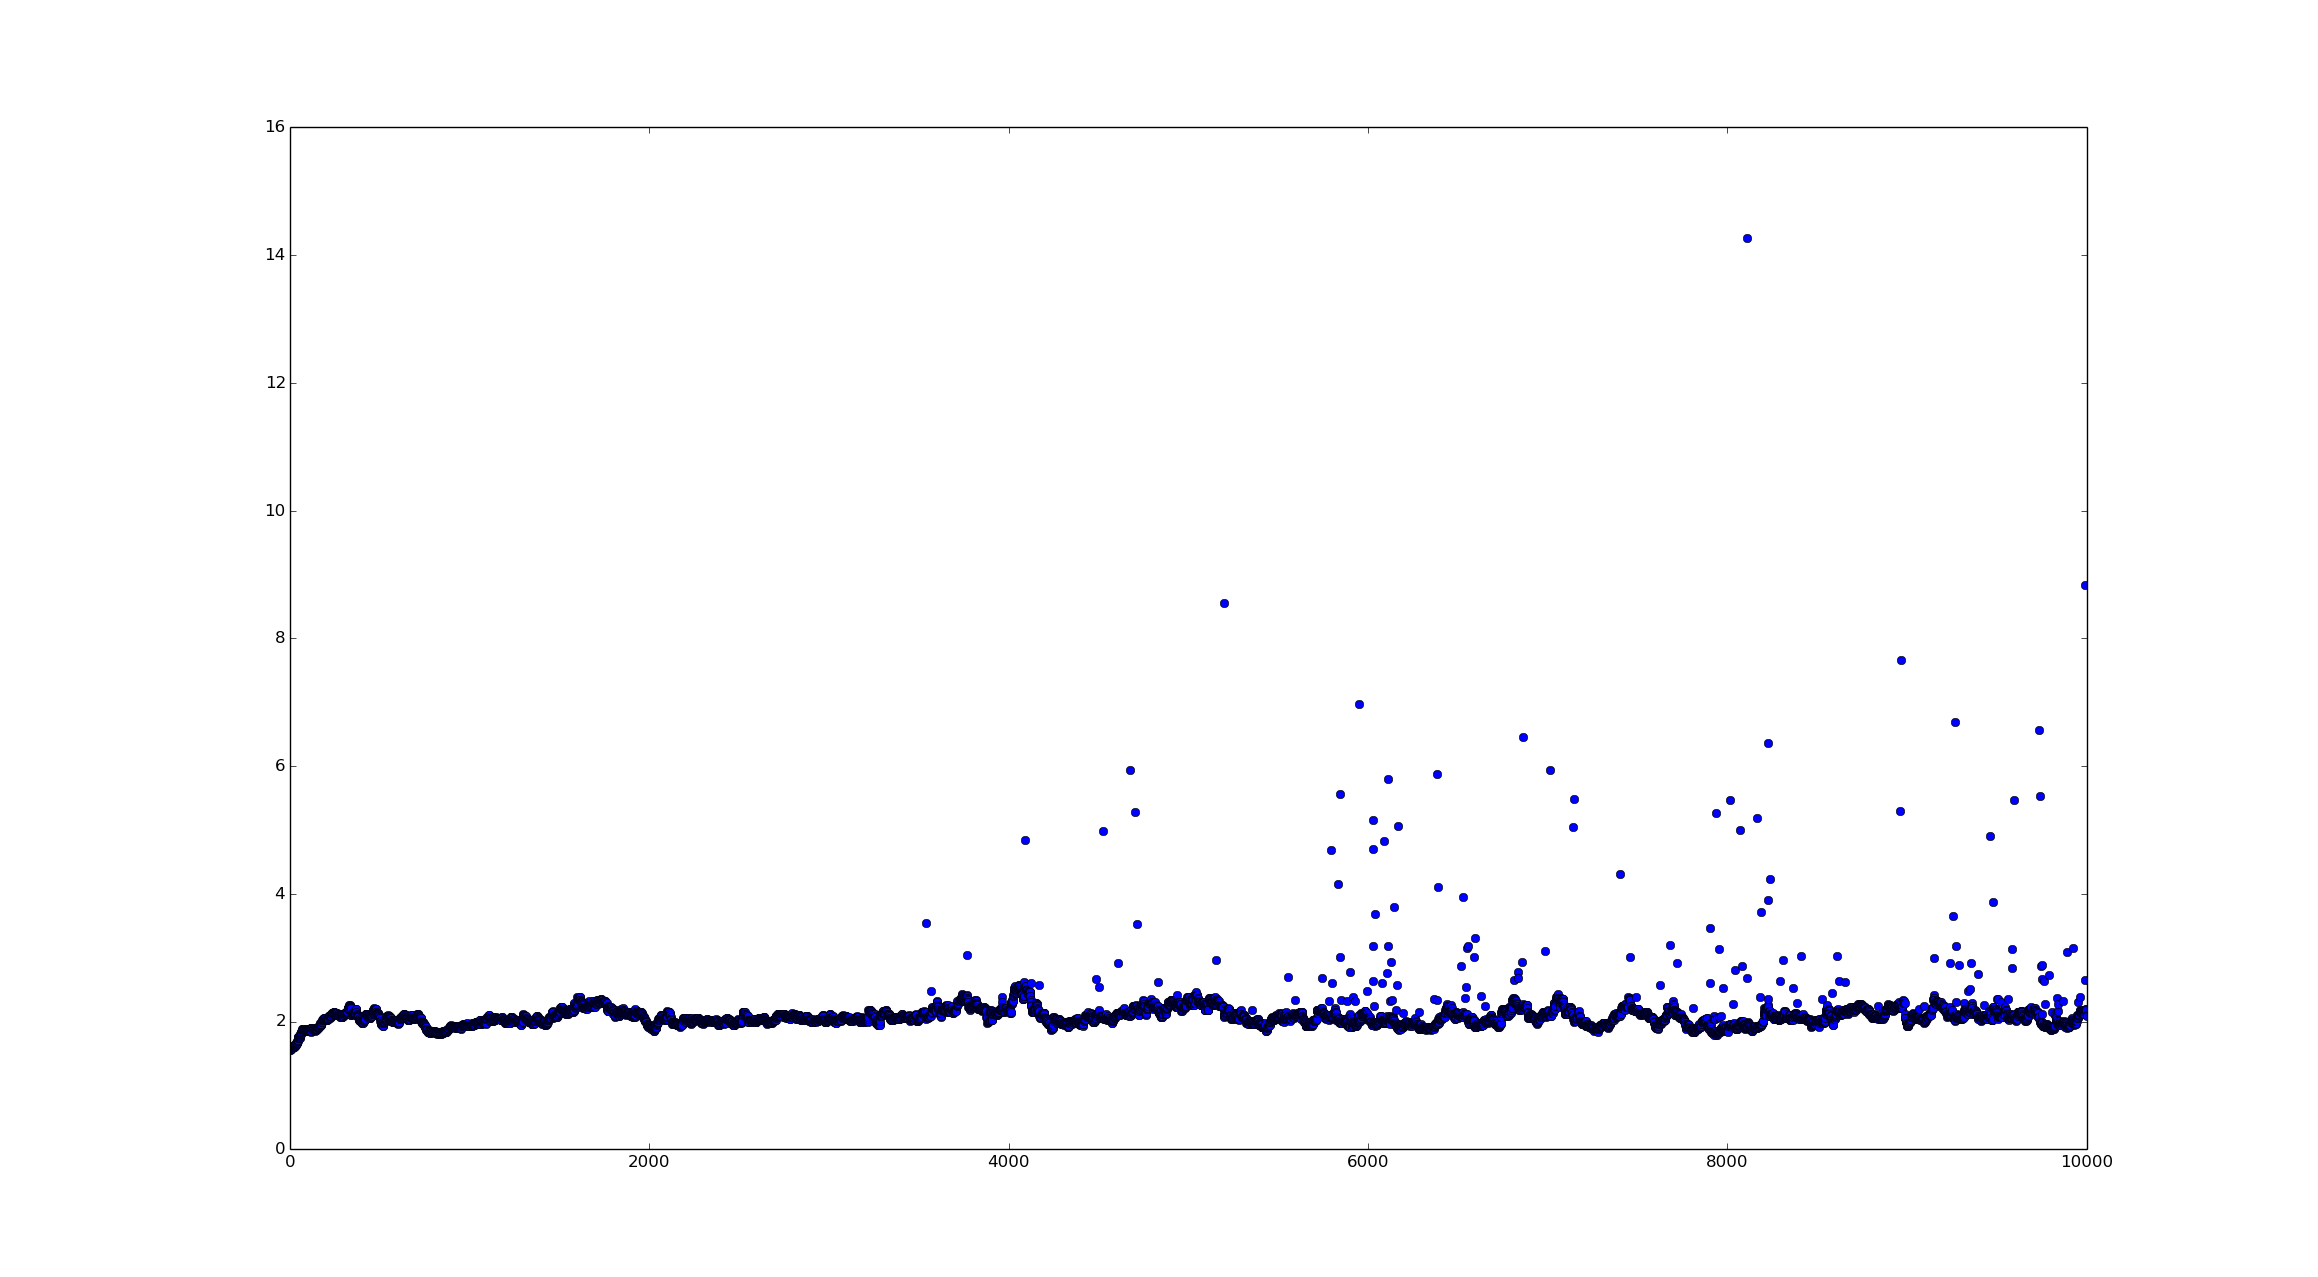
\includegraphics[width=\textwidth]{churn_stretch}
	\caption{Here we see the stretch factor (essentially embedding quality) over time as nodes exit and join the network. Removal of central nodes can often require a short period of re-ajdustment, but stretch maintains stablility over time}
\end{figure}


\subsection{Congestion and Route Diversity}
Problematically, the maintenance latency and lookup latency provided by hyperbolic embedding have an inherent disadvantage noted by previous authorities on the topic\cite{kleinberg2007geographic}. 
This latency reduction comes from having the connectivity of the distributed hash table congruent to the connectivity of the underlying scale free graph.
The degree distribution and low number of central nodes in a scale free graph forces most routing paths through high degree central nodes.

While we cannot easily decrease the maintenance overhead due to high degree, we can manage congestion using a simple mechanism.
Because DGVH maintains a list of long peers, (a size limited subset of all the "short-peers" of my "short-peers") every node connected to a central node, has a random sampling of "short-cuts" across the network that bypass high centrality nodes.
Only when the "long peers" fail to provide a reasonable alternative is a message routed to a higher centrality node.
While this dramatically reduces the network throughput required for central nodes, it should still be expected that central nodes will have a higher throughput requirement then those on the periphery of the network, but less so than the concerns of previous works\cite{kleinberg2007geographic}.
This also points out that for future work, in general, reducing the diameter of the network reduces the overall work the system has to do, and building "short cuts" around high degree nodes reduces the concentration of congestion around central nodes in a concept parallel to Kleinberg's small world networks\cite{kleinberg2000navigation}

Additional congestion avoidance behavior is trivial to implement because the DGVH mesh greedy routing can effectively route around holes, when a node is reaching congestion saturation, it can begin to respond to routing queries with a failure message, causing the forwarding algorithm to bypass the overloaded node, if the overloaded node is the only viable path to the destination, then the resulting loop the packets follow will act as an ad-hoc buffer, storing and re-trying sending messages to congested peers until they can be accepted, effectively using the network as a memory in much the same sense as a mercury delay line\cite{auerbach1949mercury}.

\begin{figure}
	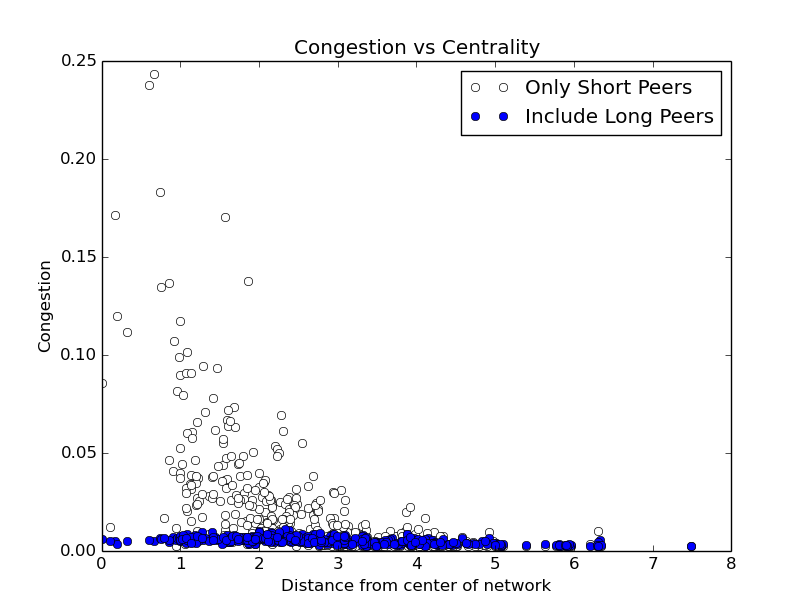
\includegraphics[width=0.5\textwidth]{radius_vs_load}
	\caption{Here we see the congestion when using short peers only (approximating a scale free graph) and when utilizing randomly selected long peers.
		Using only short peers shows that central nodes handle disproportionate amounts of messages.
	}
\end{figure}

\begin{figure}
	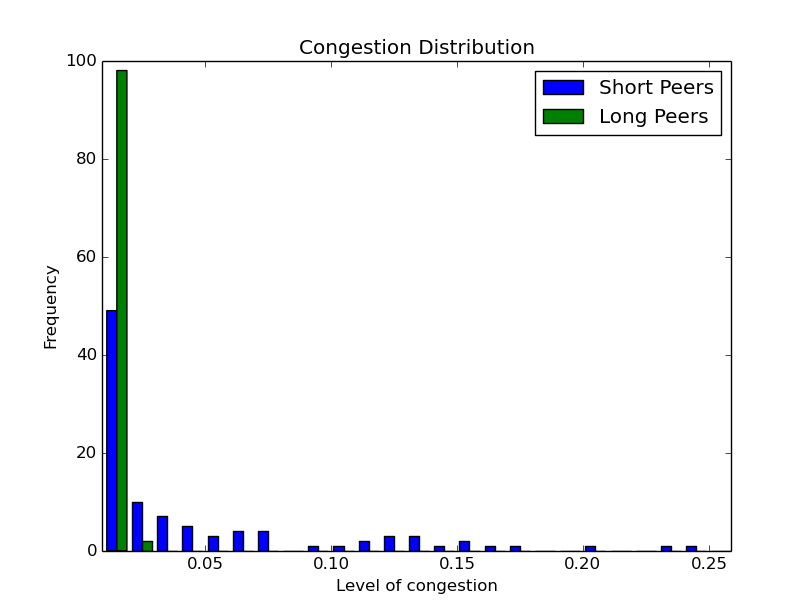
\includegraphics[width=0.5\textwidth]{congestion_4}
	\caption{Using only short peers forces more nodes, to take on higher congestion versus using long peers which globally reduces congestion.
	}
\end{figure}

\subsection{Simulation}

We simulate the greedy construction of a hyperbolic embedding and show that they produce very low latency stretch

\begin{figure}
	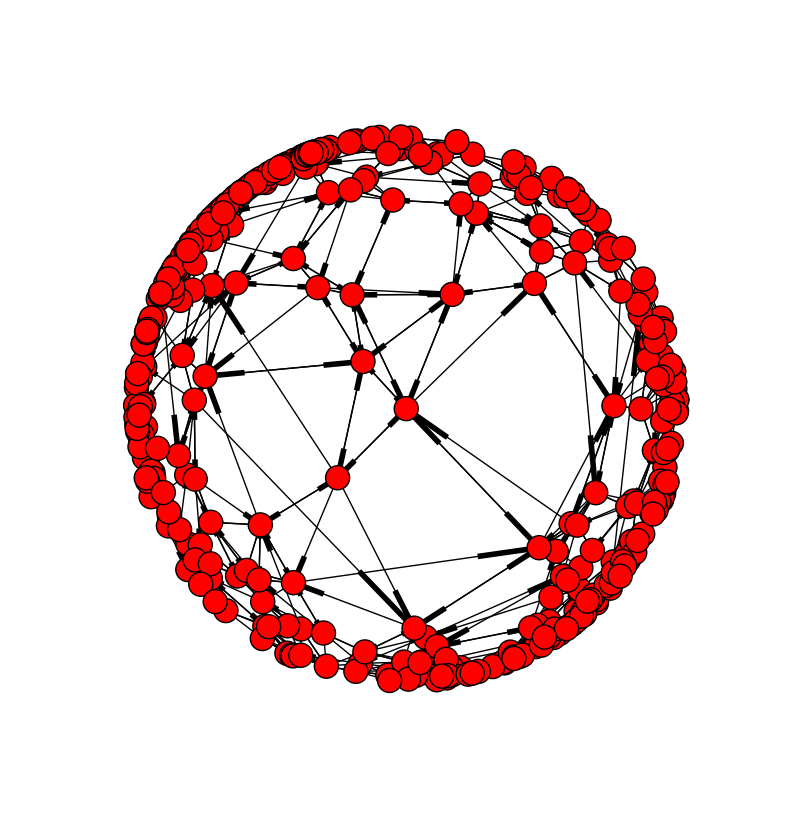
\includegraphics[width=0.5\textwidth]{disk}
	\caption{
		This is an example of the short-peer topology of a network embedded into hyperbolic space viewed through the Poincaré Disk model.
	}
\end{figure}


We simulate churn in a dynamic embedding and show that the embedding retains low latency stretch over time. We generate a 1000 node scale free graph and a size 100 overlay DHT. For 10,000 iterations we randomly select a node from the overlay and remove it, and then randomly select a node from the 1000 node underlay network and greedily insert it into the network using the join method discussed above then record and log the average route stretch.

The resulting network though churn has been totally replaced many times during the process of the simulations. 
While the quality of the simulation degrades initially from a stretch factor of 1.7, the stretch factor fluctuates around 2.0 as the simulation progresses.
Showing that greedy insertion is effective and maintaining the embedding under churn.


\section{Conclusions}
We show that a decentralized algorithm for embedding overlay networks is possible by building a greedy traversable mesh to augment a greedy embedding.
This approach is possible because we work under different assumptions than previous work, as we are attempting to approximately embed a subset of a very large scale free graph rather than a perfect embedding of an entire scale free graph.
We have shown that stretch over optimal latency is O(1) and that a finite amount of long peers can dramatically reduce network congestion and disproportionate query load in the network.

\subsubsection{Concerns and Future Work}

While we consider application of this system to practice a straightforward practice extending previous work in DGVH\cite{dgvh} usage in real systems presents a new issue.
While previous DHTs could be "optimized" to reduce effort by storing replicas of stored data at points adjacent to the host, because adjacent peers in the hyperbolic overlay are more likely to be physically close to one another, the statistical assurances provided by such robustness mechanism are weaker and such strategies should be re-examined before implementing a system similar to the one proposed in this work.







	
	\addcontentsline{toc}{chapter}{Bibliography}
	\bibliography{mine}
	\bibliographystyle{plain}
\end{document}